%% Introduction
\begin{abstract}
  En este documento se va a tratar el diseño y especificación de \ac{VIMS},
  un proyecto de ingeniería que modela, diseña y arquitecta un sistema
  conformado por un dispositivo embebido y un servidor en la nube. El
  dispositivo se conecta al vehículo y transmite, mediante redes inalámbricas,
  los datos al servidor, que hará todo el procesamiento y gestión.
  El objetivo principal es devolverle al propietario del vehículo el control
  sobre el mismo, accediendo fácilmente a los datos recogidos por el automóvil
  así como de los mensajes de error.

  Para ello, primero se recogerán datos de una muestra de conductores y
  no conductores para identificar correctamente las necesidades de los
  usuarios y ajustar mejor el producto.
  
  A continuación, se elicitarán los requisitos que permitirán posteriormente
  modelar y diseñar el sistema de forma fiel. Esta fase permite trabajar
  directamente en los diagramas que modelan el sistema, tanto a nivel de
  casuísticas como en qué estructura deberá tener. Esto es fundamental porque
  simplificará y acotará las etapas de desarrollo posteriores.

  Además, se trabajará en el estudio del modelo matemático que permite traducir
  los datos recibidos por los vehículos según el estándar \ac{OBD}--II. A su vez,
  se estudiarán las características del sistema \textit{hardware} lo que permitirá
  desarrollar y construir una placa de control que será la encargada de gestionar los
  parámetros del dispositivo \ac{VIMS}.

  Por último, se estudian las distintas tareas en tiempo real que compondrán el sistema \ac{VIMS}
  mediante el análisis de tiempo de respuesta de las mismas. Dicho análisis
  determina la planificabilidad del sistema y asegura un correcto y predecible
  funcionamiento en cualquier circunstancia.
\end{abstract}

\selectlanguage{english}
\begin{abstract}
  \ac{VIMS} design and specification project is an integral engineering development
  which designs, models and architects a whole system built with an embedded
  device and a remote cloud server. The device is attached to the driver's vehicle
  and by using wireless communication transmits the data to the remote server,
  which handles the entire processing and data generation.
  The main objective is to bring the driver's sensation back of having control
  over the vehicle, easily accessing to the entire information it provides
  alongside error messages in an easy, accessible way.

  Firstly, a quest will be done so relevant data is collected from a sample
  of drivers and non-drivers which will help identifying their needs and
  better adjusting the final product.

  Then, the requirements will be elicited which will allow the modeling
  and the design of the system in further steps of the development.
  Such step allows working directly with the diagrams that will
  model the system in both behavioral and structural manners. This is
  crucial as it will simplify and delimit the next steps of the project.

  In addition, there will be a mathematical analysis on how to translate
  the data received from the vehicle itself into human-readable information,
  based on the \ac{OBD}--II standard. Furthermore, hardware characteristics
  will be studied which will allow developing and building a PCB which will
  handle the parameters of the \ac{VIMS} device.

  Finally, a real-time task analysis will be done for \ac{VIMS} system. This will lead us
  through the definition of the tasks themselves as well as the response time
  analysis for the whole system. Thus the analysis determines if the entire
  system can be scheduled asserting a well-known, correct behavior under any
  circumstances.
\end{abstract}

\selectlanguage{spanish}


\chapter{Introducción}\label{chap:intro}
En un mundo cada vez más interconectado, hay ciertas tecnologías que se quedan
por detrás en unos campos mientras que siguen progresando en otros. Esto se ve
directamente reflejado en la industria automovilística en donde los vehículos
cada vez cuentan con mayor y mejor tecnología (como cámaras, sensores, actuadores,
etc.) pero no es directamente accesible por el usuario: mediante pantallas e
interfaces se ofrecen métodos sencillos que facilitan su uso.

\ac{VIMS} pretende ser un sistema que facilite el acceso a todos los datos que
ofrece un vehículo para generar estadísticas, descubrir patrones en la conducción
y detectar errores. De esta forma, el conductor tendrá información de primera
mano sobre el estado de su vehículo, eficiencia de su conducción así como obtener
información en tiempo real complementaria a la ya propiciada por el vehículo.

\section{Estado del arte}\label{sec:state_of_the_art}
La historia de la automoción comienza estrictamente en el siglo XIX.
Un automóvil es, por definición, un vehículo que se mueve a sí mismo
(del griego, \textit{αὐτός} ``a sí mismo'' y del latín \textit{mobilis},
``que se mueve'').

Desde los primeros modelos como la serie T, de Ford, hasta el inicio de
la fabricación de vehículos por parte de Mercedes Benz, la historia del
automovilismo ha estado llena de grandes logros y avances en un intervalo
de tiempo relativamente pequeño (figura \ref{fig:ford_model_t}):

\begin{figure}[H]
  \centering
  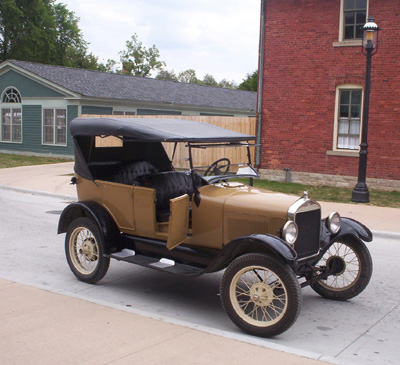
\includegraphics[width=.8\linewidth]{images/Late_model_Ford_Model_T.jpg}
  \caption{Ford modelo T del 1927 -- de Rmhermen \cite{Ford2022}.}
  \label{fig:ford_model_t}
\end{figure}

Durante aquella época, el ``mejor'' mecanismo de descubrimiento de
problemas era con algunos medidores y, sobre todo, por intuición:
sonidos del motor, olores extraños, \dots

No fue hasta los años 60 en donde los vehículos empezaron a incorporar
distintas interfaces con métricas que podían informar sobre el estado del
vehículo. El gran ``bum'' llegó con la expansión de la computadora, en donde
por primera vez se vio factible introducir un pequeño ordenador de 
abordo en el sistema.

En estos primeros sistemas, se incluyen indicadores del nivel de combustible,
sistema de refrigeración, presión del aceite, velocidad del motor,
temperatura del motor y otra información relativa al combustible. El
primer modelo que se conoce que incluye estos sistemas de cara a la
población en general es el Volkswagen Tipo III, en 1969 (figura \ref{fig:volkswagen_t3}):

\begin{figure}[H]
  \centering
  \includegraphics[width=.9\linewidth]{images/volkswagen_t3.jpg}
  \caption{Volkswagen Tipo III, modelo de inyección de 1969 -- de OSX - Trabajo propio \cite{VolkswagenTipo2021}.}
  \label{fig:volkswagen_t3}
\end{figure}

Pese a que supusieron un gran avance, estos primeros sistemas de
diagnóstico daban una información muy valiosa pero limitada, ya que muchos
diagnósticos seguirían siendo mediante los sentidos y las sensaciones
que le transmitiese el vehículo al mecánico. No fue hasta 1980 en donde
se implementó de forma estándar en los vehículos de \textit{General Motors}
el \ac{ALDL}, un lector de errores del coche que funcionó inicialmente a
160 baudios. Años más tarde, el sistema se refinaría usando el estándar
\ac{UART} \textit{half--duplex}, es decir, transmisión en los dos sentidos pero
no de forma simultánea (figura \ref{fig:aldl}). La principal motivación de incluir estos sistemas no fue
otra sino intentar reducir la contaminación de los vehículos teniendo
acceso a esta información \cite{SistemaOBD2Historia}.

\begin{figure}[H]
  \centering
  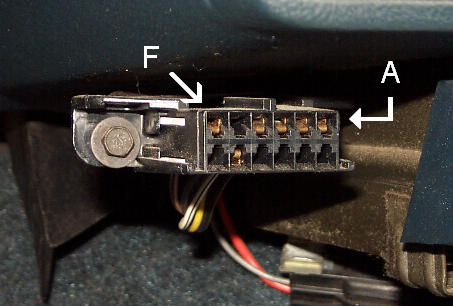
\includegraphics[width=.75\linewidth]{images/aldl.jpg}
  \caption{Conector \ac{ALDL}, creado por \textit{General Motors} antes de
  estandarizar OBD-II \cite{ReferenceManualChapter}.}
  \label{fig:aldl}
\end{figure}

No es hasta 1979 en que la \ac{SAE} recomienda crear un conector de
diagnóstico estandarizado en el mercado así como un conjunto de señales
de prueba. Finalmente, en 1991 la \ac{CARB} require que todos sus
vehículos tengan lo que sería el \ac{OBD}-I. Esta primera versión informaría
al conductor de un mal funcionamiento de alguno de los elementos del
vehículo mediante un \ac{MIL}, un indicador luminoso de fallos. Sin
embargo, solo se monitorizaban ciertos componentes relacionados con las
emisiones y no estaban calibrados \cite{SistemaOBD2Historia}.

Por ende, impulsado por las alertas \textit{smog} y por una fuerte regulación, en 1994
la \ac{CARB} obligó a todos los vehículos fabricados y vendidos a partir de 1996 incluir
el \ac{OBD}-II. Esto supuso un gran impulso en los mecanismos de monitorización de los
vehículos ya que además se estandarizó tanto el conector como los protocolos recomendados
por la \ac{SAE}. Tiempo más tarde, el Gobierno de los Estados Unidos aplicó la misma
medida a todos los vehículos del país \cite{SistemaOBD2Historia}.

Esta medida llegaría a Europa en 1998, según la Directiva 98/69EG, que obligaba a
todos los vehículos europeos a incluir dicho conector. Específicamente, los
automóviles de gasolina debían empezar a equiparlo en los modelos del año 2000; en el año 2003
para vehículos diésel; y en el año 2005 para camiones \cite{SistemaOBD2Historia}.

\subsection*{OBD--II}
\ac{OBD}--II es la segunda generación del sistema de diagnósticos de abordo, sucesor
de \ac{OBD}--I y su principal función es la de avisar al conductor cuando las
emisiones del vehículo son en torno a $1.5$ veces mayores de las diseñadas. A
diferencia de \ac{OBD}--I, \ac{OBD}--II también detecta fallos eléctricos, químicos
y mecánicos que puedan afectar al nivel de emisiones del vehículo (un caso típico
era un fallo químico del catalizador, indetectable por \ac{OBD}--I pero sí por la
segunda generación).

Este tipo de conector, al ser el primer estándar, cuenta con
múltiples interfaces que permiten conexiones mediante redes Wi-Fi, USB, Bluetooth,
etc. (cayendo pues en deshuso el protocolo de conexión por puerto serie -- RS232).
Esto se ha conseguido gracias al rápido avance de los sistemas embebidos, en donde
la combinación de \textit{software} y \textit{hardware} embebidos ha permitido que
cualquier usuario tenga acceso a este tipo de datos de forma relativamente simple
(actualmente, el conector más estandarizado es el controlador \texttt{ELM327} \cite{SistemaOBD2Historia},
figura \ref{fig:elm327}):

\begin{figure}[H]
  \centering
  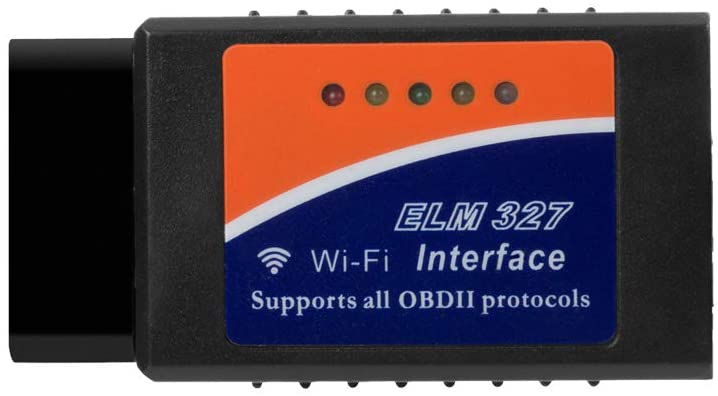
\includegraphics[width=.7\linewidth]{images/obd-ii-elm327.jpg}
  \caption{Controlador \texttt{ELM327} que cuenta con antenas Wi-Fi y Bluetooth para un acceso remoto \cite{AmazonComElm327}.}
  \label{fig:elm327}
\end{figure}

El sistema verifica todos los sensores directamente involucrados con las emisiones
del vehículo, como por ejemplo la inyección de aire al motor. Cuando algún sensor detecta
un fallo, se activa el \ac{MIL} indicando el fallo que sucede (o una combinación
de indicadores para notificar la existencia de un fallo, sin especificar exactamente
cuál).

El vehículo que incorpora un conector \ac{OBD}--II almacena la información sobre el
fallo del vehículo para que el mecánico que deba revisar el automóvil disponga de todos
los datos posibles. Por otra parte, este estándar permite una comunicación directa
con el vehículo mediante el envío de órdenes según un \ac{PID}. Por defecto, hay
una serie de \ac{PID}s estándar que la gran mayoría de vehículos deben incluir\footnote{%
Se dice ``la mayoría de vehículos'' porque hay ciertos \ac{PID}s que dependen
directamente del tipo de vehículo (a combustión, eléctrico, \dots) o del combustible
utilizado -- un vehículo eléctrico no ofrece información sobre las \ac{RPM} al igual
que un vehículo diésel no ofrece información sobre las bujías.}, pero también
los fabricantes de vehículos incluyen una serie de \ac{PID}s propios (conocidos como
\textit{\ac{PID}s propietarios}) que ofrecen información adaptada a cada vehículo
en particular y que, en principio, son privados y cerrados al público en general.

En Europa se implantó el \ac{EOBD}, la variación europea del estándar \ac{OBD}--II
implantada en el año 2000 en general. Si bien en apariencia es semejante al \ac{OBD}--II,
las diferencias radican en el \textit{software}. Por ejemplo, el estándar europeo
no monitoriza las evaporaciones del depósito de combustible; sin embargo, es más
sofisticado ya que usa ``mapas'' en las entradas de los sensores que obligan a que el
sensor se calibre empíricamente al sistema según las condiciones de operación del
motor (lo cual se traduce en que los sensores son mucho mejores pero más caros)
\cite{SistemaOBD2Historia}. Otra característica innovadora es que el sistema
europeo registra cuántos kilómetros se han recorrido desde que ha aparecido un
defecto \cite{EOBDOBD2}.

Finalmente, pero no menos importante, Japón tiene también su propio estándar denominado
\ac{JOBD}.

\subsection*{OBD--III}
El \ac{OBD}--III se espera que sea la siguiente versión del sistema que ya implementan
los coches actualmente. La principal diferencia con respecto a la versión anterior
será que el vehículo estará conectado de forma continua y emitiendo datos referentes
a las emisiones. De esta forma, se puede saber casi en el momento acerca de modificaciones
ilegales, un aumento en la contaminación del coche (signo de deterioro) y demás. No se
espera igualmente que sea un salto cualitativo ya que se sigue buscando que sea
altamente compatible con las herramientas que ya existen. Actualmente, se están
realizando pruebas en EE.UU. pero no hay cerrada ninguna fecha de estandarización
oficial por parte de los distintos continentes.

\subsection{Herramientas de monitorización y control del automóvil}
Pese al tiempo que lleva \ac{OBD}--II disponible, las herramientas existentes para
la actuación sobre un vehículo son relativamente escasas. La mayoría de modelos
presentes hoy en día en el mercado se basan directa o indirectamente en el
\texttt{ELM327}, un dispositivo de diagnóstico \ac{OBD} que cuenta con conexión
WiFi, Bluetooth y serie para la lectura local.

Por lo general, las herramientas que hay se utilizan por mecánicos o fanáticos del
sector para acceder a la información del estado del vehículo y ver los errores que
pudiera tener. Sin embargo, tras una breve documentación sobre el tema, la mayoría
de los casos buscaban directamente monitorizar en el momento el estado
del vehículo para obtener información relativa a los consumos, contaminación,
etc.

Por ejemplo, en el trabajo de Rimpas \textit{et al.} \cite{rimpasOBDIISensorDiagnostics2020}, se utiliza
un sensor \texttt{ELM327} para verificar que la información proporcionada por
el puerto del vehículo y la presentada por la telemetría presente en el mismo
(velocímetro y tacómetro) son coherentes entre sí (previa adaptación de los
valores en \textit{bytes} presentados por el conector a valores legibles). En
dicha investigación se llega a la conclusión de que el conector \ac{OBD}--II obtiene
valores fiables y consistentes tanto con los mostrados por el propio vehículo
como los proporcionados por el fabricante.

Otro tipo de investigaciones llevadas a cabo gracias a la presencia de este conector
en los automóviles es la de la caracterización de conductores y hábitos de conducción
según la telemetría reportada por el vehículo. En el estudio realizado por
Galih Hermawan y Emir Husni \cite{hermawanAcquisitionModelingEvaluating2020} se
estudia la combinación de la lectura de los sensores mediante el \ac{OBD}--II con
vehículos que presentan el sistema \ac{ADAS}.
El estudio busca identificar hábitos de conducción según la lectura de los diversos
sensores que hay en el sistema. También persigue detectar quién es el conductor que
está llevando el vehículo actualmente. En el estudio, el uso de \ac{OBD}--II junto
con los algoritmos de los \textit{k--Nearest Neighbor} (k--NN) y \textit{Naive Bayes}
consiguieron una precisión en la identificación del 100\% (
para un conjunto de datos de 10 conductores).
Por otra parte, el uso de inteligencia artificial junto con técnicas de \textit{clustering}
permitieron identificar comportamientos de los conductores al volante y relacionarlo
además con situaciones de riesgo y peligro. Además, se ha aplicado a otras características
también interesantes como detectar el tipo de calzada, predecir el tiempo de viaje,
analizar el consumo del vehículo y demás. El esquema seguido en la investigación es el
que se presenta en la figura \ref{fig:investigation-scheme}:

\begin{figure}[H]
  \centering
  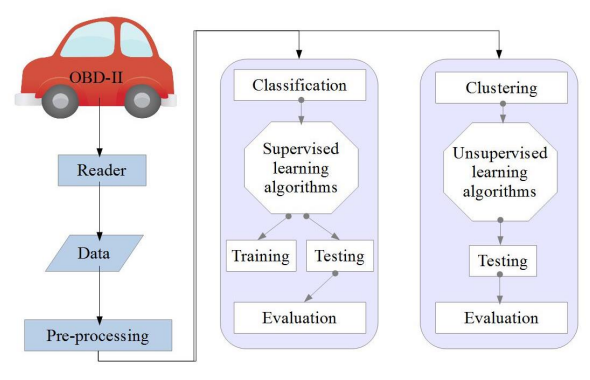
\includegraphics[width=.7\linewidth]{images/general-scheme-investigation.png}
  \caption{Esquema seguido para determinar los hábitos de conducción usando el \ac{OBD}--II \cite{hermawanAcquisitionModelingEvaluating2020}.}
  \label{fig:investigation-scheme}
\end{figure}

Por último, uno de los tipos de investigación bastante interesante realizada en los
últimos años es la de la generación de perfiles de conducción y de consumo. En el
artículo realizado por Ameen \textit{et al.} \cite{husseinaliameenDrivingBehaviourIdentification2021}
se define un sistema de clasificación del comportamiento del conductor al volante
(que es además el que se propone usar en este proyecto) el cual combina los datos
recibidos por el \ac{OBD}--II y del \ac{GPS} (figura \ref{fig:driving-behaviour}):

\begin{figure}[H]
  \centering
  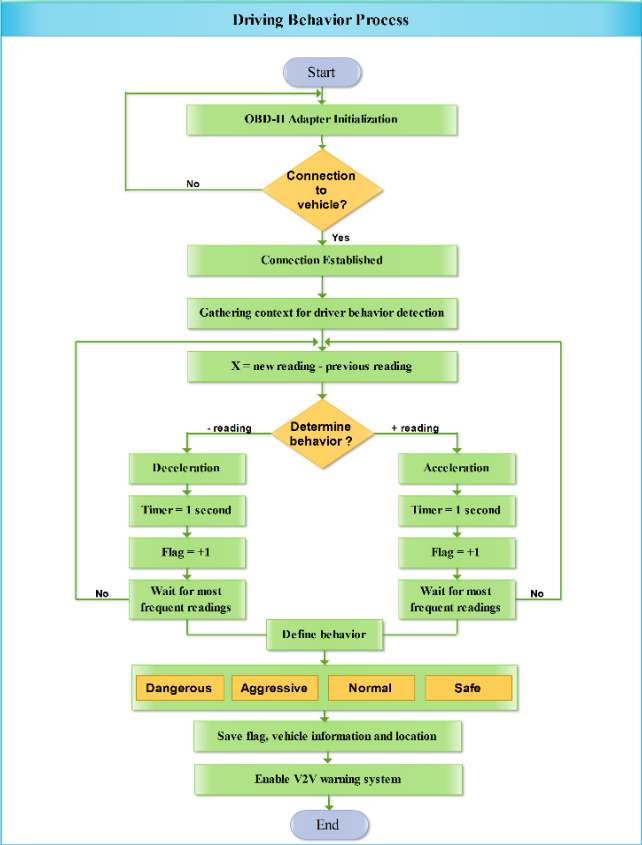
\includegraphics[width=.7\linewidth]{images/driving-behaviour-workflow.png}
  \caption{Flujo de análisis para determinar el comportamiento al volante de un conductor \cite{husseinaliameenDrivingBehaviourIdentification2021}.}
  \label{fig:driving-behaviour}
\end{figure}

Al final, el estudio concluía con los siguientes perfiles de conducción:

\begin{itemize}
  \item \textbf{Peligroso}, para una aceleración en general superior a $7\ \nicefrac{m}{s^2}$.
  \item \textbf{Agresivo}, para una aceleración entre $\left[4\ \nicefrac{m}{s^2}, 7\ \nicefrac{m}{s^2}\right)$.
  \item \textbf{Normal}, para una aceleración entre $\left[2\ \nicefrac{m}{s^2}, 4\ \nicefrac{m}{s^2}\right)$.
  \item \textbf{Seguro}, para una aceleración entre $\left[0\ \nicefrac{m}{s^2}, 2\ \nicefrac{m}{s^2}\right)$.
\end{itemize}

\section{Objetivos del desarrollo del proyecto}\label{sec:objectives}
Como se ha podido apreciar, existen multitud de aplicaciones relacionadas directa
o indirectamente con el \ac{OBD}--II, en parte por la longevidad del conector
en el mercado.

Sin embargo, todas o la gran mayoría de aplicaciones están destinadas a los profesionales
del sector, e incluso se ha aprovechado este conector para dificultar el acceso a
los datos del vehículo, habiendo de ir a un taller oficial para que puedan hacer
las reparaciones pertinentes.

Por otra parte, el parque de vehículos español es cada año más viejo debido a
diversos factores que no se van a analizar en este trabajo. Esto implica que cada
año más y más vehículos pierden el soporte por parte del fabricante y se vuelven
cada vez más costosos y complejos de mantener.

Para los no eruditos, el mundo del automóvil es el gran desconocido en donde una
serie de personas cualificadas se encargan del mantenimiento y correcto funcionamiento
del mecanismo que nos transporta por el mundo. Si bien es cierto que es necesaria
esta figura, hay una serie de buenas prácticas y actuaciones que pueden prevenir
tener que ir al mecánico de forma recurrente. Solo hace falta acceso a la información
de manera accesible.

Es por esto que nace \ac{VIMS}, un proyecto que pretende desarrollar un sistema completo
que consta de varias partes: un dispositivo embebido, un servidor y el usuario en sí
(figura \ref{fig:general-scheme}):

\begin{figure}[H]
  \centering
  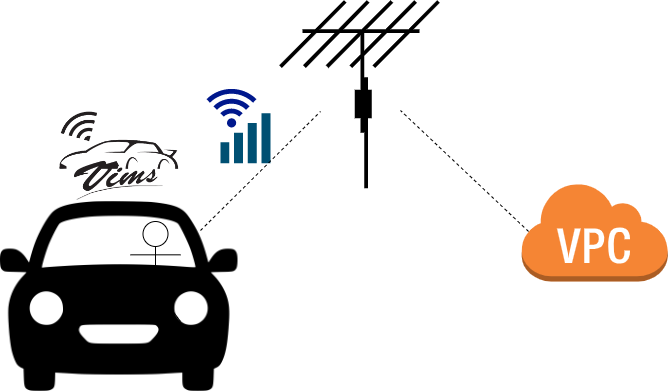
\includegraphics[width=\linewidth]{images/general-scheme.png}
  \caption{Esquema general que modela el modo de funcionamiento del sistema.}
  \label{fig:general-scheme}
\end{figure}

La idea fundamental detrás de este proyecto es la de devolverle a los usuarios
el control sobre su vehículo, ser conscientes de cómo funciona o, al menos, entender
mejor qué pueden hacer para mejorar tanto su estilo de conducción como la seguridad
al volante. De esta forma, con el dispositivo se espera también prevenir riesgos
ya que los propietarios y usuarios de los vehículos estarán informados en todo
momento de qué error pueda tener.

Como se prevé que este dispositivo sea utilizado por una gran variedad de usuarios
es crucial que sea accesible en términos de sencillez de manejo, entendimiento y
uso: evitar datos excesivamente técnicos, presentar la información más relevante
primero, etc.

Para ello, se hará uso de plataformas en la nube para gestionar, almacenar y presentar
la información al usuario y se contará con una aplicación móvil que permita un
fácil acceso a los datos del vehículo, tanto históricos como generados en el momento.

Al igual que otros trabajos previamente realizados, el proyecto se realiza sobre
las filosofías del código libre y del \textit{hardware} libre, que se traduce en
que todos los recursos (tanto físicos como \textit{software}) estarán disponibles
enteramente para cualquier persona interesada en ver cómo funciona, replicar el
proyecto por su cuenta y contar con plena potestad para mejorarlo, redistribuirlo
y trabajar con él (siempre bajo un prisma de reconocimiento al autor original
del trabajo regido por \textit{copyright}). Para ello, se ha decidido hacer uso
de la licencia MIT\footnote{Se pueden obtener más detalles sobre la licencia MIT
en la siguiente URL: \url{https://choosealicense.com/licenses/mit/}}.

\section{Metodología}\label{sec:methodology}
El proyecto que se pretende desarrollar es un proyecto de ingeniería. Esto se
traduce en que la metodología y la forma de trabajo son pilares fundamentales
en el desarrollo del mismo.

El primer paso realizado fue el de recopilar recursos e información de qué
necesitaban específicamente los usuarios. Para ello, se elaboró un cuestionario
en donde de forma general se preguntaba a conductores y no conductores qué querrían
tener en su vehículo. Los primeros sirvieron de grupo de control, los segundos para
aumentar la entropía de los datos obtenidos. El primer análisis realizado se detalla
en la sección \ref{ssec:user-req}, de la especificación de requisitos. Posteriormente,
en el punto \ref{chap:merch} se analiza en mayor profundidad los datos obtenidos
y se extraerán conclusiones.

A continuación, se realizó un estudio sobre qué plataformas y dispositivos están
accesibles de forma global para la generación y transmisión de datos. Esta fase
se centró principalmente en ``descubrir'' variantes del modelo ESP32 que incluyesen
ciertas antenas para permitir una mayor conectividad. Tras valorar diversas opciones,
se decidió usar el LILYGO T-SIM7000G ESP32 que incluye soporte de forma nativa para
tarjetas microSD, antena \ac{LTE}, alimentación externa por batería, antena \ac{GPS}, WiFi y
Bluetooth.

Una vez se decidió que dispositivo físico se iba a utilizar, se comenzó con el desarrollo
de los distintos diagramas que modelan el sistema, tanto lógicos como de diseño. Esta
parte fue crucial para asentar las bases de lo que será el proyecto y ha permitido seguir
el avance del mismo.

Por último, se realizó el serigrafiado de la placa y se comenzó la implementación
física de los diseños realizados. Sin embargo, esta etapa no se ha podido completar
por distintos contratiempos que se comentan en más detalle en el punto \ref{chap:planification}.


%% Product description
\chapter{Estructura del proyecto}\label{chap:structure}
El desarrollo del sistema \ac{VIMS} es un proceso multidisciplinar en el que se deben
desarrollar varias áreas de conocimiento. Este proyecto se ha postulado como
un desarrollo integral de ingeniería y es por eso por lo que está dividido en
varios bloques que conforman un factor clave en el desarrollo del mismo.

En este proyecto existen diversos bloques diferenciados: un estudio de mercado y de
las características de los usuarios, un estudio matemático asociado a la lectura de
valores y adecuación del \textit{hardware}, el proceso de diseño \textit{hardware}
en sí, el diseño \textit{software} del sistema y el análisis de planificación del mismo.

\begin{itemize}
  \item El estudio de mercado pretende averiguar y formalizar las necesidades de los
  conductores y usuarios de la vía. Es la primera aproximación y facilita la
  delimitación del producto y, sobre todo, ofrecerle al usuario final algo de utilidad
  y que pueda necesitar.
  \item El estudio matemático se encarga de investigar la ``traducción'' de los
  valores recibidos por el vehículo (según los datos asociados al estudio de mercado
  realizado con anterioridad).
  \item El diseño \textit{software} modela principalmente cómo se va a estructurar
  el sistema y cómo debe comportarse ante los distintos eventos que puede recibir.
  Esta fase conlleva realizar diagramas lógicos y de diseño del sistema en su conjunto.
  \item El diseño \textit{hardware} conlleva tanto el estudio de los componentes del
  sistema así como de las restricciones físicas del mismo. Además, en esta sección
  también se introduce el diseño 3D de la caja que alojará la placa.
  \item El análisis de planificabilidad complementa el diseño \textit{software}
  y estudia si el sistema es planificable. En los requisitos no se define \ac{VIMS}
  como un sistema en tiempo real, pero la cantidad de componentes que contiene y las
  acciones que tiene que realizar requieren del uso de subrutinas y de una planificación
  previa para asegurar un correcto funcionamiento del mismo.
\end{itemize}

Es importante detallar que pese a que el sistema se compone de varios componentes,
son dos los principales que lo caracterizan:

\begin{enumerate}
  \item La placa, \ac{VIMS}, que va embebida en los vehículos del sistema. Se encarga
  de toda la lectura, adaptación y emisión de datos. Además, cuenta con soporte para
  poder realizar una transmisión de la información a un dispositivo asociado mediante
  redes \ac{PAN}.
  \item El servidor \textit{cloud}, el ``cerebro'' encargado de recibir las tramas,
  los datos y la información relativa a las placas \ac{VIMS}, los dispositivos de
  usuario y demás componentes. Además, tiene la responsabilidad de ofrecer a los
  usuarios una \ac{GUI}, generar información relevante a partir de los datos (como
  estadísticas), gestionar las suscripciones y enviar periódicamente la información
  al usuario.
\end{enumerate}

\section{Estudio de mercado}\label{chap:merch}
Para el desarrollo de este proyecto, se hizo un estudio de mercado tanto de los
consumidores como de sus características, además de una evaluación exhaustiva
de qué les gustaría tener en su vehículo.

Este proyecto pretende en un futuro salir a mercado y suplir características que los
usuarios echan en falta en sus correspondientes medios de transporte. Como en principio
funciona con cualquier vehículo que cuente con \ac{OBD}--II, las respuestas no se han
limitado a aquellos conductores que condujesen turismos sino cualquier tipo de
automóvil: motocicleta, camión, etc.

Es importante destacar que el estudio tiene varios sesgos que han restringido
y delimitado las respuestas que se han registrado:

\begin{enumerate}
  \item Se ha realizado un cuestionario usando Google Forms, una plataforma de Google
        que permite preparar una serie de preguntas y respuestas y aplicar ciertos
        filtros sobre ellas. Por ejemplo, para aquellos que dijeron ser conductores,
        se hicieron preguntas diferentes frente a quienes no lo fueran.

        Esto permite obtener datos más fidedignos y acotados según la población que
        respondiera. Sin embargo, tiene una limitación implícita: restringe el acceso
        a aquellos con conocimientos ``suficientes'' acerca de la plataforma. Pese
        a que el producto pretende ser lo más accesible posible, no hay que olvidar
        que este tipo de tecnologías permanecen desconocidas para una gran parte
        de la población con escasos conocimientos acerca de Internet o de las
        nuevas tecnologías. Se comentará más adelante, pero esto se ve reflejado
        principalmente en la edad media de quienes respondieron el cuestionario.

        Por otra parte, al ser un cuestionario aparece otra limitación implícita
        y es la validación y verificación de las respuestas: se confía en la buena
        fe de los participantes y en la calidad de sus respuestas. Igualmente, se
        desarrolló el cuestionario junto con una psicóloga que ayudó a definir
        preguntas cerradas e incluir ciertas respuestas de control. Por otra parte,
        se usó el propio mecanismo que ofrece este servicio de Google para ordenar
        aleatoriamente las respuestas del cuestionario (y que eso sirviese también
        como control).

  \item Los encuestados fueron contactados principalmente por la red social Twitter,
        mediante la difusión con ``me gusta'' y ``retweet''. También se usaron otros
        medios de comunicación (como el correo UPM y Telegram/WhatsApp), pero el
        mayoritario fue el ya mencionado. Nuevamente, esto introduce un sesgo tanto
        por edad como por accesibilidad.

  \item Junto con la encuesta, se realizó un sorteo entre aquellos que respondiesen
        a la misma de un cheque regalo de Amazon valorado en 20\EUR{}. Si bien este
        incentivo pudiera resultar interesante, puede resultar también en un nuevo
        sesgo en donde personas que o bien no compren en Amazon o bien no sepan
        lo que es no quisieran hacer el cuestionario.

        Además, se plantea la casuística en que ciertas personas quisieran responder
        al cuestionario solo por el cheque de Amazon, sin importar la calidad de
        las respuestas, ``ensuciando'' los resultados obtenidos y quitándole credibilidad
        al cuestionario en sí.

        Esto se analizará posteriormente junto con las respuestas recibidas y las
        preguntas de control introducidas.

  \item El cuestionario, al ser relativamente exhaustivo, pudo echar para atrás a muchos
        posibles encuestados ya que se estima que el tiempo medio para realizarlo es del
        orden de 10/15 minutos. A parte del daño evidente de tener menos muestra con la
        que trabajar, este posible suceso reduciría también la variedad de la población
        y la calidad del estudio realizado.
\end{enumerate}

La primera pregunta que se realizó a los encuestados era si eran conductores o no.
Los datos revelan que el $72.7\%$ ($16$) de los encuestados son conductores, mientras que el
$27.3\%$ ($6$) restantes no, del total que fueron $22$ (figura \ref{fig:drivers-nodrivers}):

\begin{figure}[H]
  \centering
  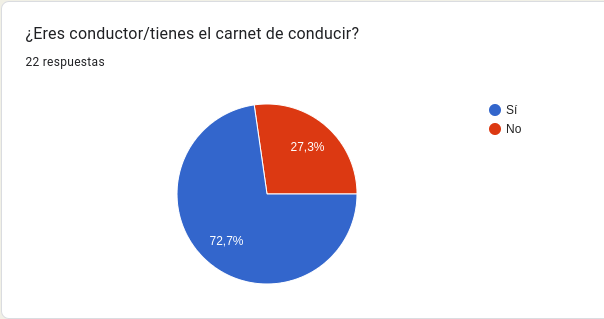
\includegraphics[width=\linewidth]{images/drivers-nodrivers.png}
  \caption{Gráfico de tarta que muestra quiénes de los encuestados son conductores ($72.7\%$) y quiénes no ($27.3\%$).}
  \label{fig:drivers-nodrivers}
\end{figure}

Sobre aquellos que dijeron ser conductores, se preguntó acerca de los años que
llevaban con carnet de conducir, así como los tipos de carnet de conducir que tenían
los encuestados.

Se vio que un $68.8\%$ tenía el carnet desde hace 3 años o más ($11$ encuestados
en particular); un $12.5\%$ tenía el carnet desde hace solo un año ($2$ encuestados)
y el restante, en su mayoría, tenía el carnet desde hace menos de un año. Esto se ve
reflejado en el histograma \ref{fig:carnet-time-hist}:

\begin{figure}[H]
  \centering
  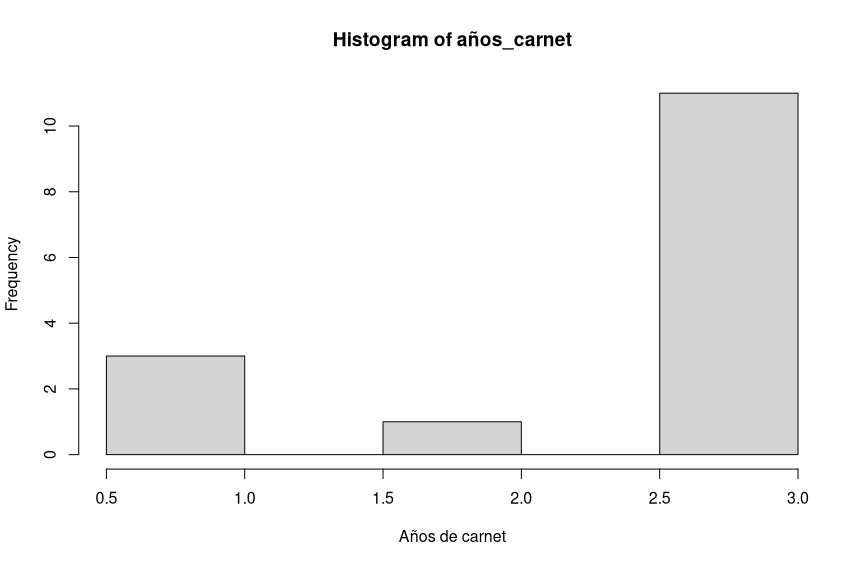
\includegraphics[width=\linewidth]{images/carnet-time.png}
  \caption{Histograma que muestra los años de carnet de los encuestados.}
  \label{fig:carnet-time-hist}
\end{figure}

Con respecto a los tipos de carnet, el $100\%$ de los encuestados (que dijeron ser
conductores) tiene el carnet tipo B. Se vio además que el $18.8\%$ tiene además los
carnets relativos a las motocicletas (muy posiblemente, los encuestados tienen el
carnet tipo ``A'' que les habilita automáticamente para aquellos de menor nivel,
como el AM, A1 y A2); y únicamente un encuestado tiene el carnet tipo C, que permite
conducir camiones.

Una restricción que se comentó con anterioridad era la edad media de los participantes.
Esta pregunta se realizó por dos motivos:

\begin{enumerate}
  \item Definir estadísticamente la edad media de la población para una posterior evaluación
        de su longevidad y experiencia tanto en la conducción como en la posible
        compra-venta de vehículos.
  \item Diferenciar, definir y clasificar los encuestados por grupos de edad y descubrir
        posibles sesgos y restricciones en las respuestas para un posterior análisis
        sobre la causa de dichos sesgos y restricciones.
\end{enumerate}

Es necesario decir que solo se preguntó por la edad a aquellas personas que respondieron
afirmativamente a ser conductores. Esto se hizo así debido a que sus respuestas han
conformado el dato más relativo a la hora de realizar la investigación, y se hace así
también estadísticamente.

Se tiene pues que:

\begin{equation}\label{eq:ages}
  \left\{\begin{aligned}
    X_{min}               & = 19     \\
    \bar{X}               & = 30     \\
    Mediana\left(X\right) & = 26.5   \\
    S\left(X\right)       & = 10.564 \\
    X_{max}               & = 55
  \end{aligned}\right.
\end{equation}

Se construyó además un gráfico de tarta (figura \ref{fig:ages}) que muestra cómo
quedan distribuidas las edades de los participantes:

\begin{figure}[H]
  \centering
  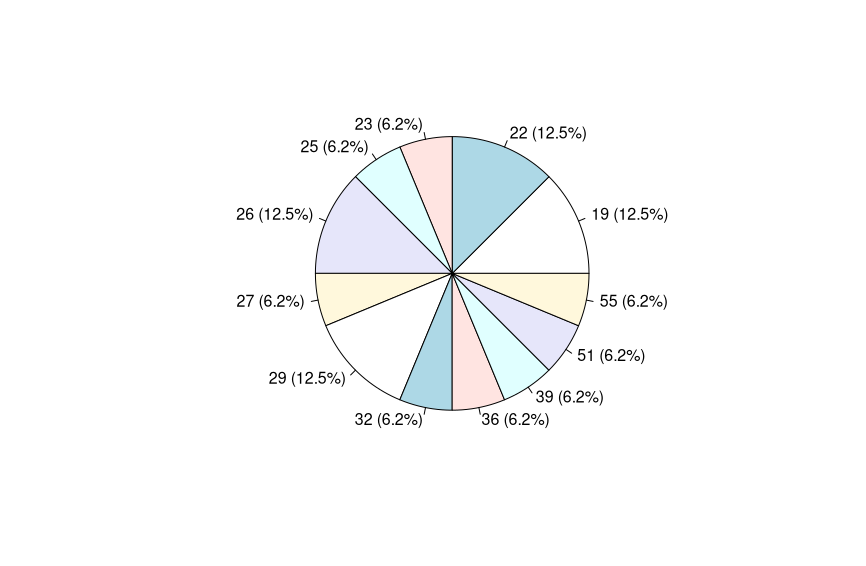
\includegraphics[width=\linewidth]{images/ages-pie.png}
  \caption{Gráfico de tarta que muestra la distribución de edades (valor previo al paréntesis) y su frecuencia en porcentaje.}
  \label{fig:ages}
\end{figure}

Como se puede ver en la ecuación \ref{eq:ages}, la distancia entre los valores
mínimo y máximo es de $36$ puntos. Sin embargo, los valores de la media $\left(\bar{X}\right)$
y la mediana $\left(Mediana\left(X\right)\right)$ muestran que la distribución está
bastante centrada en torno a la media, con una desviación estándar $\left(S\left(X\right)\right)$
de $\approx\pm10.564$.

Es interesante notar los tres grandes bloques presentes en la figura \ref{fig:ages}
que evidencian lo que se venía indicando anteriormente: en proporción, a la encuesta
ha accedido más población joven que adulta. Mismamente, solo el porcentaje de personas
encuestadas con edad por debajo de los 26 años es del $49.9\%$, casi la mitad de
los encuestados. Ampliando dicho margen hasta los 36 años, el porcentaje crece hasta
el $81 \%$.

Este dato se puede ver también reflejado en la distribución de los cuartiles, en donde
se tiene que:

\begin{equation}\label{eq:age-quartiles}
  \left\{
  \begin{aligned}
    Q_1 & = 22.75 \\
    Q_3 & = 33.00
  \end{aligned}
  \right.
\end{equation}

Como se puede apreciar en la ecuación \ref{eq:age-quartiles}, la distribución de
cuartiles está en un rango de edad por debajo de los 33 años para el $75\%$ de la
muestra, indicativo nuevamente de una población encuestada joven.

Destacan dos datos sobre los demás en donde los encuestados tienen 51 y 55 años
respectivamente. De este caso en particular se hablará posteriormente, pero cabe
destacar que sus respuestas fueron las más pobres en cuanto a contenido (sobre todo
en aquellas que sirvieron de control), seguramente debido al formato del
cuestionario, fatiga tras responder las secciones anteriores, etc.

Una vez se indagó acerca de la información que identifica a la muestra, se preguntó
directamente por el vehículo con el que contaban así como las características del
mismo. Para esta sección, se han dividido las preguntas en tres categorías:
\textit{básico}, \textit{habitual} y \textit{premium}. Dichas categorías se crean
según el porcentaje de uso habitual mundial de las características que se
enumeran en la tabla \ref{tab:car-specs}:

\begin{table}[H]
  \centering
  \begin{tabular}{|c|c|c|}
    \hline
    \textbf{Básico}          & \textbf{Habitual}            & \textit{\textbf{Premium}} \\
    \hline\hline
    Control de crucero       & Pantalla táctil              & Asistente virtual         \\
    Limitador de velocidad   & GPS                          & Aplicación móvil          \\
    Cámara de visión trasera & Detección de ángulos muertos & Cámara \textit{on-board}  \\
    Botón de arranque        & Android Auto                 &                           \\
    \hline
  \end{tabular}
  \caption{Tabla de distribución de las características de los vehículos, preguntado en el cuestionario.}
  \label{tab:car-specs}
\end{table}

Tras el cuestionario, las frecuencias obtenidas fueron:

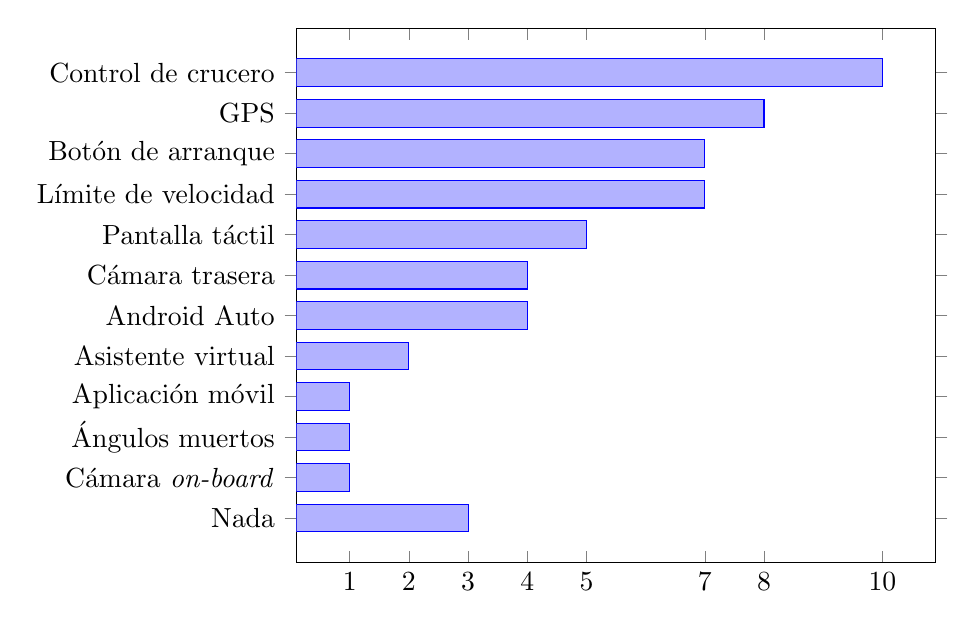
\begin{tikzpicture}
  \begin{axis} [%
      xbar,
      width=.8\linewidth,
      ytick=data,
      yticklabels={%
          Nada,
          Cámara \textit{on-board},
          Ángulos muertos,
          Aplicación móvil,
          Asistente virtual,
          Android Auto,
          Cámara trasera,
          Pantalla táctil,
          Límite de velocidad,
          Botón de arranque,
          GPS,
          Control de crucero,
        },
      xtick=data,
    ]
    \addplot coordinates {
        (3, 0)
        (1, 1)
        (1, 2)
        (1, 3)
        (2, 4)
        (4, 5)
        (4, 6)
        (5, 7)
        (7, 8)
        (7, 9)
        (8, 10)
        (10, 11)
      };
  \end{axis}
\end{tikzpicture}

\section{Estudio matemático}\label{sec:maths}
\section{Diseño \textit{software}}\label{sec:software}
\section{Diseño \textit{hardware}}\label{sec:hardware}
\section{Análisis de planificabilidad}\label{sec:rt-analysis}

%% Requirements
\chapter{Especificación de requisitos}\label{chap:requirements}
%% Introduction
\begin{abstract}
  En este documento se va a tratar el diseño y especificación de \ac{VIMS},
  un proyecto de ingeniería que modela, diseña y arquitecta un sistema
  conformado por un dispositivo embebido y un servidor en la nube. El
  dispositivo se conecta al vehículo y transmite, mediante redes inalámbricas,
  los datos al servidor, que hará todo el procesamiento y gestión.
  El objetivo principal es devolverle al propietario del vehículo el control
  sobre el mismo, accediendo fácilmente a los datos recogidos por el automóvil
  así como de los mensajes de error.

  Para ello, primero se recogerán datos de una muestra de conductores y
  no conductores para identificar correctamente las necesidades de los
  usuarios y ajustar mejor el producto.
  
  A continuación, se elicitarán los requisitos que permitirán posteriormente
  modelar y diseñar el sistema de forma fiel. Esta fase permite trabajar
  directamente en los diagramas que modelan el sistema, tanto a nivel de
  casuísticas como en qué estructura deberá tener. Esto es fundamental porque
  simplificará y acotará las etapas de desarrollo posteriores.

  Además, se trabajará en el estudio del modelo matemático que permite traducir
  los datos recibidos por los vehículos según el estándar \ac{OBD}--II. A su vez,
  se estudiarán las características del sistema \textit{hardware} lo que permitirá
  desarrollar y construir una placa de control que será la encargada de gestionar los
  parámetros del dispositivo \ac{VIMS}.

  Por último, se estudian las distintas tareas en tiempo real que compondrán el sistema \ac{VIMS}
  mediante el análisis de tiempo de respuesta de las mismas. Dicho análisis
  determina la planificabilidad del sistema y asegura un correcto y predecible
  funcionamiento en cualquier circunstancia.
\end{abstract}

\selectlanguage{english}
\begin{abstract}
  \ac{VIMS} design and specification project is an integral engineering development
  which designs, models and architects a whole system built with an embedded
  device and a remote cloud server. The device is attached to the driver's vehicle
  and by using wireless communication transmits the data to the remote server,
  which handles the entire processing and data generation.
  The main objective is to bring the driver's sensation back of having control
  over the vehicle, easily accessing to the entire information it provides
  alongside error messages in an easy, accessible way.

  Firstly, a quest will be done so relevant data is collected from a sample
  of drivers and non-drivers which will help identifying their needs and
  better adjusting the final product.

  Then, the requirements will be elicited which will allow the modeling
  and the design of the system in further steps of the development.
  Such step allows working directly with the diagrams that will
  model the system in both behavioral and structural manners. This is
  crucial as it will simplify and delimit the next steps of the project.

  In addition, there will be a mathematical analysis on how to translate
  the data received from the vehicle itself into human-readable information,
  based on the \ac{OBD}--II standard. Furthermore, hardware characteristics
  will be studied which will allow developing and building a PCB which will
  handle the parameters of the \ac{VIMS} device.

  Finally, a real-time task analysis will be done for \ac{VIMS} system. This will lead us
  through the definition of the tasks themselves as well as the response time
  analysis for the whole system. Thus the analysis determines if the entire
  system can be scheduled asserting a well-known, correct behavior under any
  circumstances.
\end{abstract}

\selectlanguage{spanish}


\chapter{Introducción}\label{chap:intro}
En un mundo cada vez más interconectado, hay ciertas tecnologías que se quedan
por detrás en unos campos mientras que siguen progresando en otros. Esto se ve
directamente reflejado en la industria automovilística en donde los vehículos
cada vez cuentan con mayor y mejor tecnología (como cámaras, sensores, actuadores,
etc.) pero no es directamente accesible por el usuario: mediante pantallas e
interfaces se ofrecen métodos sencillos que facilitan su uso.

\ac{VIMS} pretende ser un sistema que facilite el acceso a todos los datos que
ofrece un vehículo para generar estadísticas, descubrir patrones en la conducción
y detectar errores. De esta forma, el conductor tendrá información de primera
mano sobre el estado de su vehículo, eficiencia de su conducción así como obtener
información en tiempo real complementaria a la ya propiciada por el vehículo.

\section{Estado del arte}\label{sec:state_of_the_art}
La historia de la automoción comienza estrictamente en el siglo XIX.
Un automóvil es, por definición, un vehículo que se mueve a sí mismo
(del griego, \textit{αὐτός} ``a sí mismo'' y del latín \textit{mobilis},
``que se mueve'').

Desde los primeros modelos como la serie T, de Ford, hasta el inicio de
la fabricación de vehículos por parte de Mercedes Benz, la historia del
automovilismo ha estado llena de grandes logros y avances en un intervalo
de tiempo relativamente pequeño (figura \ref{fig:ford_model_t}):

\begin{figure}[H]
  \centering
  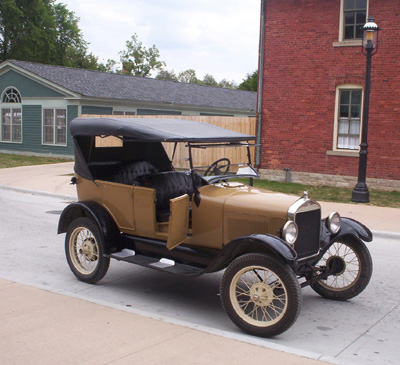
\includegraphics[width=.8\linewidth]{images/Late_model_Ford_Model_T.jpg}
  \caption{Ford modelo T del 1927 -- de Rmhermen \cite{Ford2022}.}
  \label{fig:ford_model_t}
\end{figure}

Durante aquella época, el ``mejor'' mecanismo de descubrimiento de
problemas era con algunos medidores y, sobre todo, por intuición:
sonidos del motor, olores extraños, \dots

No fue hasta los años 60 en donde los vehículos empezaron a incorporar
distintas interfaces con métricas que podían informar sobre el estado del
vehículo. El gran ``bum'' llegó con la expansión de la computadora, en donde
por primera vez se vio factible introducir un pequeño ordenador de 
abordo en el sistema.

En estos primeros sistemas, se incluyen indicadores del nivel de combustible,
sistema de refrigeración, presión del aceite, velocidad del motor,
temperatura del motor y otra información relativa al combustible. El
primer modelo que se conoce que incluye estos sistemas de cara a la
población en general es el Volkswagen Tipo III, en 1969 (figura \ref{fig:volkswagen_t3}):

\begin{figure}[H]
  \centering
  \includegraphics[width=.9\linewidth]{images/volkswagen_t3.jpg}
  \caption{Volkswagen Tipo III, modelo de inyección de 1969 -- de OSX - Trabajo propio \cite{VolkswagenTipo2021}.}
  \label{fig:volkswagen_t3}
\end{figure}

Pese a que supusieron un gran avance, estos primeros sistemas de
diagnóstico daban una información muy valiosa pero limitada, ya que muchos
diagnósticos seguirían siendo mediante los sentidos y las sensaciones
que le transmitiese el vehículo al mecánico. No fue hasta 1980 en donde
se implementó de forma estándar en los vehículos de \textit{General Motors}
el \ac{ALDL}, un lector de errores del coche que funcionó inicialmente a
160 baudios. Años más tarde, el sistema se refinaría usando el estándar
\ac{UART} \textit{half--duplex}, es decir, transmisión en los dos sentidos pero
no de forma simultánea (figura \ref{fig:aldl}). La principal motivación de incluir estos sistemas no fue
otra sino intentar reducir la contaminación de los vehículos teniendo
acceso a esta información \cite{SistemaOBD2Historia}.

\begin{figure}[H]
  \centering
  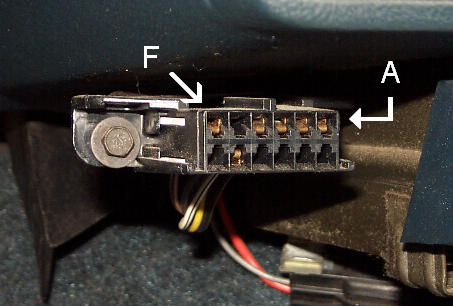
\includegraphics[width=.75\linewidth]{images/aldl.jpg}
  \caption{Conector \ac{ALDL}, creado por \textit{General Motors} antes de
  estandarizar OBD-II \cite{ReferenceManualChapter}.}
  \label{fig:aldl}
\end{figure}

No es hasta 1979 en que la \ac{SAE} recomienda crear un conector de
diagnóstico estandarizado en el mercado así como un conjunto de señales
de prueba. Finalmente, en 1991 la \ac{CARB} require que todos sus
vehículos tengan lo que sería el \ac{OBD}-I. Esta primera versión informaría
al conductor de un mal funcionamiento de alguno de los elementos del
vehículo mediante un \ac{MIL}, un indicador luminoso de fallos. Sin
embargo, solo se monitorizaban ciertos componentes relacionados con las
emisiones y no estaban calibrados \cite{SistemaOBD2Historia}.

Por ende, impulsado por las alertas \textit{smog} y por una fuerte regulación, en 1994
la \ac{CARB} obligó a todos los vehículos fabricados y vendidos a partir de 1996 incluir
el \ac{OBD}-II. Esto supuso un gran impulso en los mecanismos de monitorización de los
vehículos ya que además se estandarizó tanto el conector como los protocolos recomendados
por la \ac{SAE}. Tiempo más tarde, el Gobierno de los Estados Unidos aplicó la misma
medida a todos los vehículos del país \cite{SistemaOBD2Historia}.

Esta medida llegaría a Europa en 1998, según la Directiva 98/69EG, que obligaba a
todos los vehículos europeos a incluir dicho conector. Específicamente, los
automóviles de gasolina debían empezar a equiparlo en los modelos del año 2000; en el año 2003
para vehículos diésel; y en el año 2005 para camiones \cite{SistemaOBD2Historia}.

\subsection*{OBD--II}
\ac{OBD}--II es la segunda generación del sistema de diagnósticos de abordo, sucesor
de \ac{OBD}--I y su principal función es la de avisar al conductor cuando las
emisiones del vehículo son en torno a $1.5$ veces mayores de las diseñadas. A
diferencia de \ac{OBD}--I, \ac{OBD}--II también detecta fallos eléctricos, químicos
y mecánicos que puedan afectar al nivel de emisiones del vehículo (un caso típico
era un fallo químico del catalizador, indetectable por \ac{OBD}--I pero sí por la
segunda generación).

Este tipo de conector, al ser el primer estándar, cuenta con
múltiples interfaces que permiten conexiones mediante redes Wi-Fi, USB, Bluetooth,
etc. (cayendo pues en deshuso el protocolo de conexión por puerto serie -- RS232).
Esto se ha conseguido gracias al rápido avance de los sistemas embebidos, en donde
la combinación de \textit{software} y \textit{hardware} embebidos ha permitido que
cualquier usuario tenga acceso a este tipo de datos de forma relativamente simple
(actualmente, el conector más estandarizado es el controlador \texttt{ELM327} \cite{SistemaOBD2Historia},
figura \ref{fig:elm327}):

\begin{figure}[H]
  \centering
  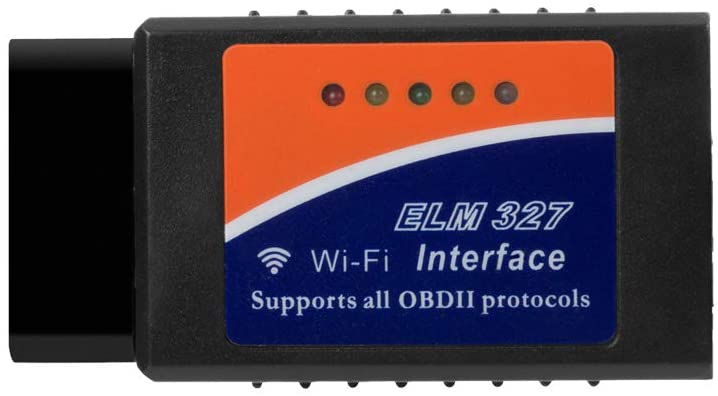
\includegraphics[width=.7\linewidth]{images/obd-ii-elm327.jpg}
  \caption{Controlador \texttt{ELM327} que cuenta con antenas Wi-Fi y Bluetooth para un acceso remoto \cite{AmazonComElm327}.}
  \label{fig:elm327}
\end{figure}

El sistema verifica todos los sensores directamente involucrados con las emisiones
del vehículo, como por ejemplo la inyección de aire al motor. Cuando algún sensor detecta
un fallo, se activa el \ac{MIL} indicando el fallo que sucede (o una combinación
de indicadores para notificar la existencia de un fallo, sin especificar exactamente
cuál).

El vehículo que incorpora un conector \ac{OBD}--II almacena la información sobre el
fallo del vehículo para que el mecánico que deba revisar el automóvil disponga de todos
los datos posibles. Por otra parte, este estándar permite una comunicación directa
con el vehículo mediante el envío de órdenes según un \ac{PID}. Por defecto, hay
una serie de \ac{PID}s estándar que la gran mayoría de vehículos deben incluir\footnote{%
Se dice ``la mayoría de vehículos'' porque hay ciertos \ac{PID}s que dependen
directamente del tipo de vehículo (a combustión, eléctrico, \dots) o del combustible
utilizado -- un vehículo eléctrico no ofrece información sobre las \ac{RPM} al igual
que un vehículo diésel no ofrece información sobre las bujías.}, pero también
los fabricantes de vehículos incluyen una serie de \ac{PID}s propios (conocidos como
\textit{\ac{PID}s propietarios}) que ofrecen información adaptada a cada vehículo
en particular y que, en principio, son privados y cerrados al público en general.

En Europa se implantó el \ac{EOBD}, la variación europea del estándar \ac{OBD}--II
implantada en el año 2000 en general. Si bien en apariencia es semejante al \ac{OBD}--II,
las diferencias radican en el \textit{software}. Por ejemplo, el estándar europeo
no monitoriza las evaporaciones del depósito de combustible; sin embargo, es más
sofisticado ya que usa ``mapas'' en las entradas de los sensores que obligan a que el
sensor se calibre empíricamente al sistema según las condiciones de operación del
motor (lo cual se traduce en que los sensores son mucho mejores pero más caros)
\cite{SistemaOBD2Historia}. Otra característica innovadora es que el sistema
europeo registra cuántos kilómetros se han recorrido desde que ha aparecido un
defecto \cite{EOBDOBD2}.

Finalmente, pero no menos importante, Japón tiene también su propio estándar denominado
\ac{JOBD}.

\subsection*{OBD--III}
El \ac{OBD}--III se espera que sea la siguiente versión del sistema que ya implementan
los coches actualmente. La principal diferencia con respecto a la versión anterior
será que el vehículo estará conectado de forma continua y emitiendo datos referentes
a las emisiones. De esta forma, se puede saber casi en el momento acerca de modificaciones
ilegales, un aumento en la contaminación del coche (signo de deterioro) y demás. No se
espera igualmente que sea un salto cualitativo ya que se sigue buscando que sea
altamente compatible con las herramientas que ya existen. Actualmente, se están
realizando pruebas en EE.UU. pero no hay cerrada ninguna fecha de estandarización
oficial por parte de los distintos continentes.

\subsection{Herramientas de monitorización y control del automóvil}
Pese al tiempo que lleva \ac{OBD}--II disponible, las herramientas existentes para
la actuación sobre un vehículo son relativamente escasas. La mayoría de modelos
presentes hoy en día en el mercado se basan directa o indirectamente en el
\texttt{ELM327}, un dispositivo de diagnóstico \ac{OBD} que cuenta con conexión
WiFi, Bluetooth y serie para la lectura local.

Por lo general, las herramientas que hay se utilizan por mecánicos o fanáticos del
sector para acceder a la información del estado del vehículo y ver los errores que
pudiera tener. Sin embargo, tras una breve documentación sobre el tema, la mayoría
de los casos buscaban directamente monitorizar en el momento el estado
del vehículo para obtener información relativa a los consumos, contaminación,
etc.

Por ejemplo, en el trabajo de Rimpas \textit{et al.} \cite{rimpasOBDIISensorDiagnostics2020}, se utiliza
un sensor \texttt{ELM327} para verificar que la información proporcionada por
el puerto del vehículo y la presentada por la telemetría presente en el mismo
(velocímetro y tacómetro) son coherentes entre sí (previa adaptación de los
valores en \textit{bytes} presentados por el conector a valores legibles). En
dicha investigación se llega a la conclusión de que el conector \ac{OBD}--II obtiene
valores fiables y consistentes tanto con los mostrados por el propio vehículo
como los proporcionados por el fabricante.

Otro tipo de investigaciones llevadas a cabo gracias a la presencia de este conector
en los automóviles es la de la caracterización de conductores y hábitos de conducción
según la telemetría reportada por el vehículo. En el estudio realizado por
Galih Hermawan y Emir Husni \cite{hermawanAcquisitionModelingEvaluating2020} se
estudia la combinación de la lectura de los sensores mediante el \ac{OBD}--II con
vehículos que presentan el sistema \ac{ADAS}.
El estudio busca identificar hábitos de conducción según la lectura de los diversos
sensores que hay en el sistema. También persigue detectar quién es el conductor que
está llevando el vehículo actualmente. En el estudio, el uso de \ac{OBD}--II junto
con los algoritmos de los \textit{k--Nearest Neighbor} (k--NN) y \textit{Naive Bayes}
consiguieron una precisión en la identificación del 100\% (
para un conjunto de datos de 10 conductores).
Por otra parte, el uso de inteligencia artificial junto con técnicas de \textit{clustering}
permitieron identificar comportamientos de los conductores al volante y relacionarlo
además con situaciones de riesgo y peligro. Además, se ha aplicado a otras características
también interesantes como detectar el tipo de calzada, predecir el tiempo de viaje,
analizar el consumo del vehículo y demás. El esquema seguido en la investigación es el
que se presenta en la figura \ref{fig:investigation-scheme}:

\begin{figure}[H]
  \centering
  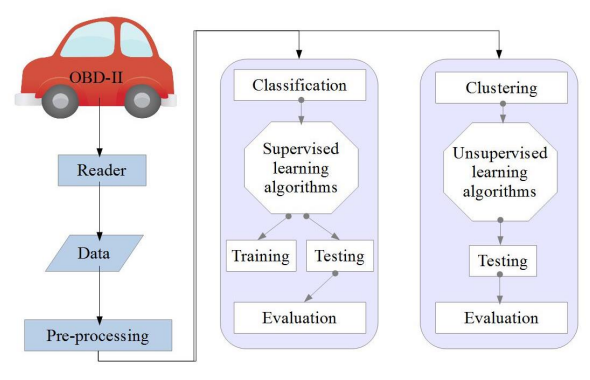
\includegraphics[width=.7\linewidth]{images/general-scheme-investigation.png}
  \caption{Esquema seguido para determinar los hábitos de conducción usando el \ac{OBD}--II \cite{hermawanAcquisitionModelingEvaluating2020}.}
  \label{fig:investigation-scheme}
\end{figure}

Por último, uno de los tipos de investigación bastante interesante realizada en los
últimos años es la de la generación de perfiles de conducción y de consumo. En el
artículo realizado por Ameen \textit{et al.} \cite{husseinaliameenDrivingBehaviourIdentification2021}
se define un sistema de clasificación del comportamiento del conductor al volante
(que es además el que se propone usar en este proyecto) el cual combina los datos
recibidos por el \ac{OBD}--II y del \ac{GPS} (figura \ref{fig:driving-behaviour}):

\begin{figure}[H]
  \centering
  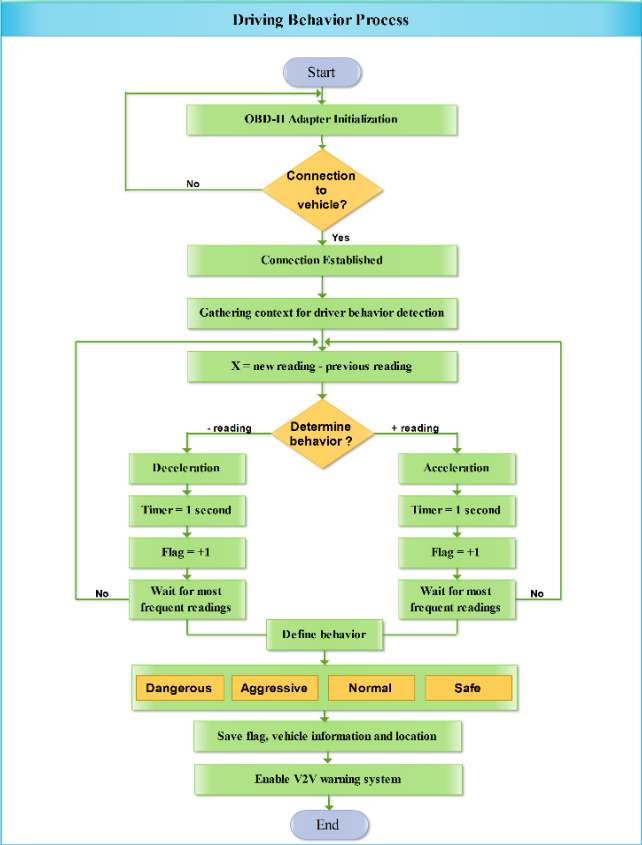
\includegraphics[width=.7\linewidth]{images/driving-behaviour-workflow.png}
  \caption{Flujo de análisis para determinar el comportamiento al volante de un conductor \cite{husseinaliameenDrivingBehaviourIdentification2021}.}
  \label{fig:driving-behaviour}
\end{figure}

Al final, el estudio concluía con los siguientes perfiles de conducción:

\begin{itemize}
  \item \textbf{Peligroso}, para una aceleración en general superior a $7\ \nicefrac{m}{s^2}$.
  \item \textbf{Agresivo}, para una aceleración entre $\left[4\ \nicefrac{m}{s^2}, 7\ \nicefrac{m}{s^2}\right)$.
  \item \textbf{Normal}, para una aceleración entre $\left[2\ \nicefrac{m}{s^2}, 4\ \nicefrac{m}{s^2}\right)$.
  \item \textbf{Seguro}, para una aceleración entre $\left[0\ \nicefrac{m}{s^2}, 2\ \nicefrac{m}{s^2}\right)$.
\end{itemize}

\section{Objetivos del desarrollo del proyecto}\label{sec:objectives}
Como se ha podido apreciar, existen multitud de aplicaciones relacionadas directa
o indirectamente con el \ac{OBD}--II, en parte por la longevidad del conector
en el mercado.

Sin embargo, todas o la gran mayoría de aplicaciones están destinadas a los profesionales
del sector, e incluso se ha aprovechado este conector para dificultar el acceso a
los datos del vehículo, habiendo de ir a un taller oficial para que puedan hacer
las reparaciones pertinentes.

Por otra parte, el parque de vehículos español es cada año más viejo debido a
diversos factores que no se van a analizar en este trabajo. Esto implica que cada
año más y más vehículos pierden el soporte por parte del fabricante y se vuelven
cada vez más costosos y complejos de mantener.

Para los no eruditos, el mundo del automóvil es el gran desconocido en donde una
serie de personas cualificadas se encargan del mantenimiento y correcto funcionamiento
del mecanismo que nos transporta por el mundo. Si bien es cierto que es necesaria
esta figura, hay una serie de buenas prácticas y actuaciones que pueden prevenir
tener que ir al mecánico de forma recurrente. Solo hace falta acceso a la información
de manera accesible.

Es por esto que nace \ac{VIMS}, un proyecto que pretende desarrollar un sistema completo
que consta de varias partes: un dispositivo embebido, un servidor y el usuario en sí
(figura \ref{fig:general-scheme}):

\begin{figure}[H]
  \centering
  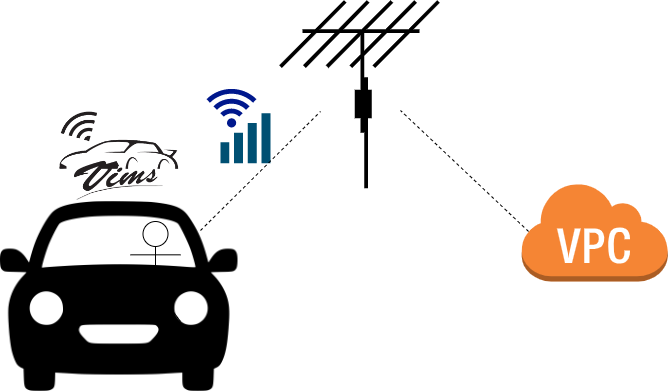
\includegraphics[width=\linewidth]{images/general-scheme.png}
  \caption{Esquema general que modela el modo de funcionamiento del sistema.}
  \label{fig:general-scheme}
\end{figure}

La idea fundamental detrás de este proyecto es la de devolverle a los usuarios
el control sobre su vehículo, ser conscientes de cómo funciona o, al menos, entender
mejor qué pueden hacer para mejorar tanto su estilo de conducción como la seguridad
al volante. De esta forma, con el dispositivo se espera también prevenir riesgos
ya que los propietarios y usuarios de los vehículos estarán informados en todo
momento de qué error pueda tener.

Como se prevé que este dispositivo sea utilizado por una gran variedad de usuarios
es crucial que sea accesible en términos de sencillez de manejo, entendimiento y
uso: evitar datos excesivamente técnicos, presentar la información más relevante
primero, etc.

Para ello, se hará uso de plataformas en la nube para gestionar, almacenar y presentar
la información al usuario y se contará con una aplicación móvil que permita un
fácil acceso a los datos del vehículo, tanto históricos como generados en el momento.

Al igual que otros trabajos previamente realizados, el proyecto se realiza sobre
las filosofías del código libre y del \textit{hardware} libre, que se traduce en
que todos los recursos (tanto físicos como \textit{software}) estarán disponibles
enteramente para cualquier persona interesada en ver cómo funciona, replicar el
proyecto por su cuenta y contar con plena potestad para mejorarlo, redistribuirlo
y trabajar con él (siempre bajo un prisma de reconocimiento al autor original
del trabajo regido por \textit{copyright}). Para ello, se ha decidido hacer uso
de la licencia MIT\footnote{Se pueden obtener más detalles sobre la licencia MIT
en la siguiente URL: \url{https://choosealicense.com/licenses/mit/}}.

\section{Metodología}\label{sec:methodology}
El proyecto que se pretende desarrollar es un proyecto de ingeniería. Esto se
traduce en que la metodología y la forma de trabajo son pilares fundamentales
en el desarrollo del mismo.

El primer paso realizado fue el de recopilar recursos e información de qué
necesitaban específicamente los usuarios. Para ello, se elaboró un cuestionario
en donde de forma general se preguntaba a conductores y no conductores qué querrían
tener en su vehículo. Los primeros sirvieron de grupo de control, los segundos para
aumentar la entropía de los datos obtenidos. El primer análisis realizado se detalla
en la sección \ref{ssec:user-req}, de la especificación de requisitos. Posteriormente,
en el punto \ref{chap:merch} se analiza en mayor profundidad los datos obtenidos
y se extraerán conclusiones.

A continuación, se realizó un estudio sobre qué plataformas y dispositivos están
accesibles de forma global para la generación y transmisión de datos. Esta fase
se centró principalmente en ``descubrir'' variantes del modelo ESP32 que incluyesen
ciertas antenas para permitir una mayor conectividad. Tras valorar diversas opciones,
se decidió usar el LILYGO T-SIM7000G ESP32 que incluye soporte de forma nativa para
tarjetas microSD, antena \ac{LTE}, alimentación externa por batería, antena \ac{GPS}, WiFi y
Bluetooth.

Una vez se decidió que dispositivo físico se iba a utilizar, se comenzó con el desarrollo
de los distintos diagramas que modelan el sistema, tanto lógicos como de diseño. Esta
parte fue crucial para asentar las bases de lo que será el proyecto y ha permitido seguir
el avance del mismo.

Por último, se realizó el serigrafiado de la placa y se comenzó la implementación
física de los diseños realizados. Sin embargo, esta etapa no se ha podido completar
por distintos contratiempos que se comentan en más detalle en el punto \ref{chap:planification}.


%% Product description
\chapter{Estructura del proyecto}\label{chap:structure}
El desarrollo del sistema \ac{VIMS} es un proceso multidisciplinar en el que se deben
desarrollar varias áreas de conocimiento. Este proyecto se ha postulado como
un desarrollo integral de ingeniería y es por eso por lo que está dividido en
varios bloques que conforman un factor clave en el desarrollo del mismo.

En este proyecto existen diversos bloques diferenciados: un estudio de mercado y de
las características de los usuarios, un estudio matemático asociado a la lectura de
valores y adecuación del \textit{hardware}, el proceso de diseño \textit{hardware}
en sí, el diseño \textit{software} del sistema y el análisis de planificación del mismo.

\begin{itemize}
  \item El estudio de mercado pretende averiguar y formalizar las necesidades de los
  conductores y usuarios de la vía. Es la primera aproximación y facilita la
  delimitación del producto y, sobre todo, ofrecerle al usuario final algo de utilidad
  y que pueda necesitar.
  \item El estudio matemático se encarga de investigar la ``traducción'' de los
  valores recibidos por el vehículo (según los datos asociados al estudio de mercado
  realizado con anterioridad).
  \item El diseño \textit{software} modela principalmente cómo se va a estructurar
  el sistema y cómo debe comportarse ante los distintos eventos que puede recibir.
  Esta fase conlleva realizar diagramas lógicos y de diseño del sistema en su conjunto.
  \item El diseño \textit{hardware} conlleva tanto el estudio de los componentes del
  sistema así como de las restricciones físicas del mismo. Además, en esta sección
  también se introduce el diseño 3D de la caja que alojará la placa.
  \item El análisis de planificabilidad complementa el diseño \textit{software}
  y estudia si el sistema es planificable. En los requisitos no se define \ac{VIMS}
  como un sistema en tiempo real, pero la cantidad de componentes que contiene y las
  acciones que tiene que realizar requieren del uso de subrutinas y de una planificación
  previa para asegurar un correcto funcionamiento del mismo.
\end{itemize}

Es importante detallar que pese a que el sistema se compone de varios componentes,
son dos los principales que lo caracterizan:

\begin{enumerate}
  \item La placa, \ac{VIMS}, que va embebida en los vehículos del sistema. Se encarga
  de toda la lectura, adaptación y emisión de datos. Además, cuenta con soporte para
  poder realizar una transmisión de la información a un dispositivo asociado mediante
  redes \ac{PAN}.
  \item El servidor \textit{cloud}, el ``cerebro'' encargado de recibir las tramas,
  los datos y la información relativa a las placas \ac{VIMS}, los dispositivos de
  usuario y demás componentes. Además, tiene la responsabilidad de ofrecer a los
  usuarios una \ac{GUI}, generar información relevante a partir de los datos (como
  estadísticas), gestionar las suscripciones y enviar periódicamente la información
  al usuario.
\end{enumerate}

\section{Estudio de mercado}\label{sec:merch}
Para el desarrollo de este proyecto, se hizo un estudio de mercado tanto de los
consumidores como de sus características, además de una evaluación exhaustiva
de qué les gustaría tener en su vehículo.

Este proyecto pretende en un futuro salir a mercado y suplir características que los
usuarios echan en falta en sus correspondientes medios de transporte. Como en principio
funciona con cualquier vehículo que cuente con \ac{OBD}--II, las respuestas no se han
limitado a aquellos conductores que condujesen turismos sino cualquier tipo de
automóvil: motocicleta, camión, etc.

Es importante destacar que el estudio tiene varios sesgos que han restringido
y delimitado las respuestas que se han registrado:

\begin{enumerate}
  \item Se ha realizado un cuestionario usando Google Forms, una plataforma de Google
        que permite preparar una serie de preguntas y respuestas y aplicar ciertos
        filtros sobre ellas. Por ejemplo, para aquellos que dijeron ser conductores,
        se hicieron preguntas diferentes frente a quienes no lo fueran.

        Esto permite obtener datos más fidedignos y acotados según la población que
        respondiera. Sin embargo, tiene una limitación implícita: restringe el acceso
        a aquellos con conocimientos ``suficientes'' acerca de la plataforma. Pese
        a que el producto pretende ser lo más accesible posible, no hay que olvidar
        que este tipo de tecnologías permanecen desconocidas para una gran parte
        de la población con escasos conocimientos acerca de Internet o de las
        nuevas tecnologías. Se comentará más adelante, pero esto se ve reflejado
        principalmente en la edad media de quienes respondieron el cuestionario.

        Por otra parte, al ser un cuestionario aparece otra limitación implícita
        y es la validación y verificación de las respuestas: se confía en la buena
        fe de los participantes y en la calidad de sus respuestas. Igualmente, se
        desarrolló el cuestionario junto con una psicóloga que ayudó a definir
        preguntas cerradas e incluir ciertas respuestas de control. Por otra parte,
        se usó el propio mecanismo que ofrece este servicio de Google para ordenar
        aleatoriamente las respuestas del cuestionario (y que eso sirviese también
        como control).

  \item Los encuestados fueron contactados principalmente por la red social Twitter,
        mediante la difusión con ``me gusta'' y ``retweet''. También se usaron otros
        medios de comunicación (como el correo UPM y Telegram/WhatsApp), pero el
        mayoritario fue el ya mencionado. Nuevamente, esto introduce un sesgo tanto
        por edad como por accesibilidad.

  \item Junto con la encuesta, se realizó un sorteo entre aquellos que respondiesen
        a la misma de un cheque regalo de Amazon valorado en 20\EUR{}. Si bien este
        incentivo pudiera resultar interesante, puede resultar también en un nuevo
        sesgo en donde personas que o bien no compren en Amazon o bien no sepan
        lo que es no quisieran hacer el cuestionario.

        Además, se plantea la casuística en que ciertas personas quisieran responder
        al cuestionario solo por el cheque de Amazon, sin importar la calidad de
        las respuestas, ``ensuciando'' los resultados obtenidos y quitándole credibilidad
        al cuestionario en sí.

        Esto se analizará posteriormente junto con las respuestas recibidas y las
        preguntas de control introducidas.

  \item El cuestionario, al ser relativamente exhaustivo, pudo echar para atrás a muchos
        posibles encuestados ya que se estima que el tiempo medio para realizarlo es del
        orden de 10/15 minutos. A parte del daño evidente de tener menos muestra con la
        que trabajar, este posible suceso reduciría también la variedad de la población
        y la calidad del estudio realizado.
\end{enumerate}

La primera pregunta que se realizó a los encuestados era si eran conductores o no.
Los datos revelan que el $72.7\%$ ($16$) de los encuestados son conductores, mientras que el
$27.3\%$ ($6$) restantes no, del total que fueron $22$ (figura \ref{fig:drivers-nodrivers}):

\begin{figure}[H]
  \centering
  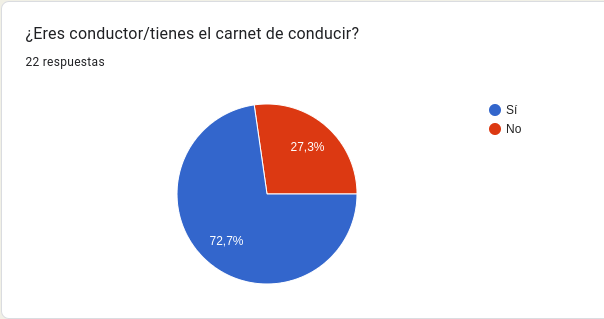
\includegraphics[width=\linewidth]{images/drivers-nodrivers.png}
  \caption{Gráfico de tarta que muestra quiénes de los encuestados son conductores ($72.7\%$) y quiénes no ($27.3\%$).}
  \label{fig:drivers-nodrivers}
\end{figure}

Sobre aquellos que dijeron ser conductores, se preguntó acerca de los años que
llevaban con carnet de conducir, así como los tipos de carnet de conducir que tenían
los encuestados.

Se vio que un $68.8\%$ tenía el carnet desde hace 3 años o más ($11$ encuestados
en particular); un $12.5\%$ tenía el carnet desde hace solo un año ($2$ encuestados)
y el restante, en su mayoría, tenía el carnet desde hace menos de un año. Esto se ve
reflejado en el histograma \ref{fig:carnet-time-hist}:

\begin{figure}[H]
  \centering
  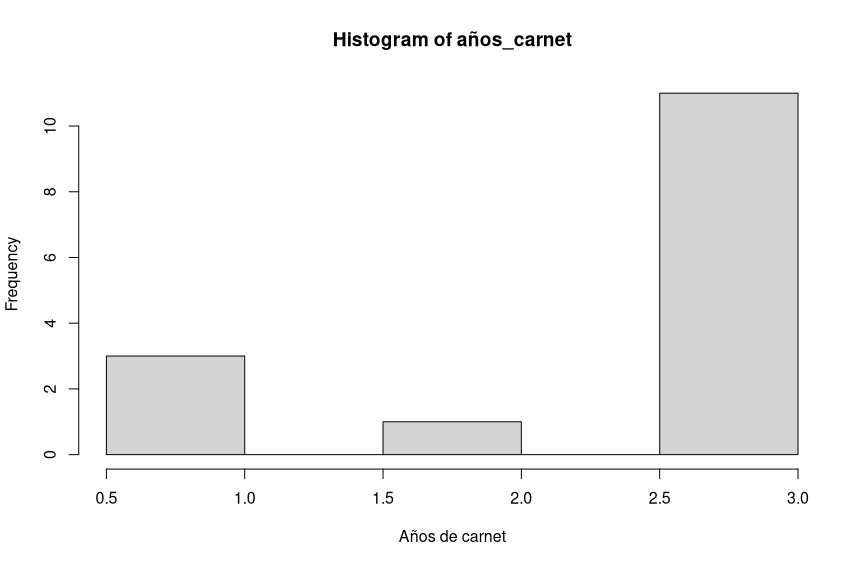
\includegraphics[width=\linewidth]{images/carnet-time.png}
  \caption{Histograma que muestra los años de carnet de los encuestados.}
  \label{fig:carnet-time-hist}
\end{figure}

Con respecto a los tipos de carnet, el $100\%$ de los encuestados (que dijeron ser
conductores) tiene el carnet tipo B. Se vio además que el $18.8\%$ tiene además los
carnets relativos a las motocicletas (muy posiblemente, los encuestados tienen el
carnet tipo ``A'' que les habilita automáticamente para aquellos de menor nivel,
como el AM, A1 y A2); y únicamente un encuestado tiene el carnet tipo C, que permite
conducir camiones.

Una restricción que se comentó con anterioridad era la edad media de los participantes.
Esta pregunta se realizó por dos motivos:

\begin{enumerate}
  \item Definir estadísticamente la edad media de la población para una posterior evaluación
        de su longevidad y experiencia tanto en la conducción como en la posible
        compra-venta de vehículos.
  \item Diferenciar, definir y clasificar los encuestados por grupos de edad y descubrir
        posibles sesgos y restricciones en las respuestas para un posterior análisis
        sobre la causa de dichos sesgos y restricciones.
\end{enumerate}

Es necesario decir que solo se preguntó por la edad a aquellas personas que respondieron
afirmativamente a ser conductores. Esto se hizo así debido a que sus respuestas han
conformado el dato más relativo a la hora de realizar la investigación, y se hace así
también estadísticamente.

Se tiene pues que:

\begin{equation}\label{eq:ages}
  \left\{\begin{aligned}
    X_{min}               & = 19     \\
    \bar{X}               & = 30     \\
    Mediana\left(X\right) & = 26.5   \\
    S\left(X\right)       & = 10.564 \\
    X_{max}               & = 55
  \end{aligned}\right.
\end{equation}

Se construyó además un gráfico de tarta (figura \ref{fig:ages}) que muestra cómo
quedan distribuidas las edades de los participantes:

\begin{figure}[H]
  \centering
  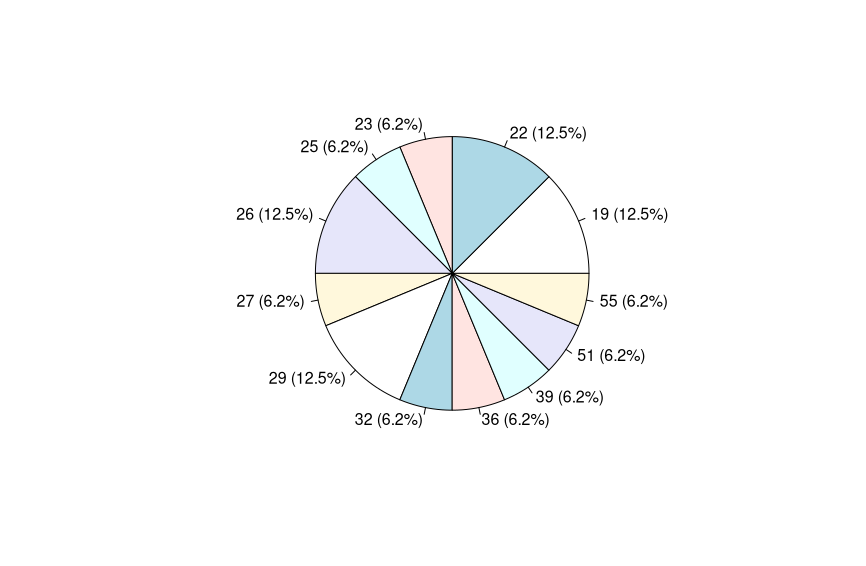
\includegraphics[width=\linewidth]{images/ages-pie.png}
  \caption{Gráfico de tarta que muestra la distribución de edades (valor previo al paréntesis) y su frecuencia en porcentaje.}
  \label{fig:ages}
\end{figure}

Como se puede ver en la ecuación \ref{eq:ages}, la distancia entre los valores
mínimo y máximo es de $36$ puntos. Sin embargo, los valores de la media $\left(\bar{X}\right)$
y la mediana $\left(Mediana\left(X\right)\right)$ muestran que la distribución está
bastante centrada en torno a la media, con una desviación estándar $\left(S\left(X\right)\right)$
de $\approx\pm10.564$.

Es interesante notar los tres grandes bloques presentes en la figura \ref{fig:ages}
que evidencian lo que se venía indicando anteriormente: en proporción, a la encuesta
ha accedido más población joven que adulta. Mismamente, solo el porcentaje de personas
encuestadas con edad por debajo de los 26 años es del $49.9\%$, casi la mitad de
los encuestados. Ampliando dicho margen hasta los 36 años, el porcentaje crece hasta
el $81 \%$.

Este dato se puede ver también reflejado en la distribución de los cuartiles, en donde
se tiene que:

\begin{equation}\label{eq:age-quartiles}
  \left\{
  \begin{aligned}
    Q_1 & = 22.75 \\
    Q_3 & = 33.00
  \end{aligned}
  \right.
\end{equation}

Como se puede apreciar en la ecuación \ref{eq:age-quartiles}, la distribución de
cuartiles está en un rango de edad por debajo de los 33 años para el $75\%$ de la
muestra, indicativo nuevamente de una población encuestada joven.

Destacan dos datos sobre los demás en donde los encuestados tienen 51 y 55 años
respectivamente. De este caso en particular se hablará posteriormente, pero cabe
destacar que sus respuestas fueron las más pobres en cuanto a contenido (sobre todo
en aquellas que sirvieron de control), seguramente debido al formato del
cuestionario, fatiga tras responder las secciones anteriores, etc.

Una vez se indagó acerca de la información que identifica a la muestra, se preguntó
directamente por el vehículo con el que contaban así como las características del
mismo. Para esta sección, se han dividido las preguntas en tres categorías:
\textit{básico}, \textit{habitual} y \textit{premium}. Dichas categorías se crean
según el porcentaje de uso habitual mundial de las características que se
enumeran en la tabla \ref{tab:car-specs}:

\begin{table}[H]
  \centering
  \begin{tabular}{|c|c|c|}
    \hline
    \textbf{Básico}          & \textbf{Habitual}            & \textit{\textbf{Premium}} \\
    \hline\hline
    Control de crucero       & Pantalla táctil              & Asistente virtual         \\
    Limitador de velocidad   & GPS                          & Aplicación móvil          \\
    Cámara de visión trasera & Detección de ángulos muertos & Cámara \textit{on-board}  \\
    Botón de arranque        & Android Auto                 &                           \\
    \hline
  \end{tabular}
  \caption{Tabla de distribución de las características de los vehículos, preguntado en el cuestionario.}
  \label{tab:car-specs}
\end{table}

Tras el cuestionario, las frecuencias obtenidas fueron:

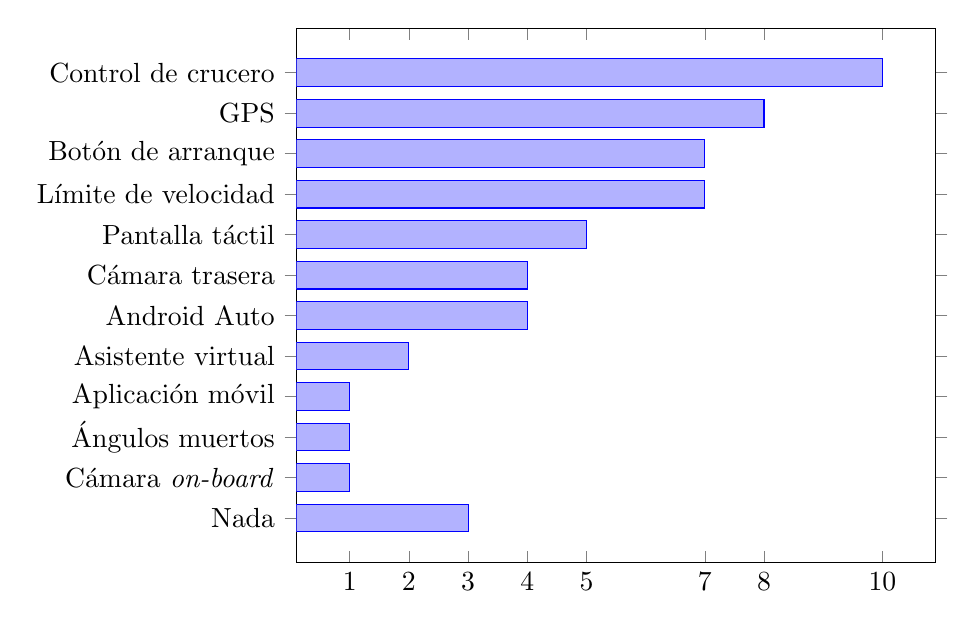
\begin{tikzpicture}
  \begin{axis} [%
      xbar,
      width=.8\linewidth,
      ytick=data,
      yticklabels={%
          Nada,
          Cámara \textit{on-board},
          Ángulos muertos,
          Aplicación móvil,
          Asistente virtual,
          Android Auto,
          Cámara trasera,
          Pantalla táctil,
          Límite de velocidad,
          Botón de arranque,
          GPS,
          Control de crucero,
        },
      xtick=data,
    ]
    \addplot coordinates {
        (3, 0)
        (1, 1)
        (1, 2)
        (1, 3)
        (2, 4)
        (4, 5)
        (4, 6)
        (5, 7)
        (7, 8)
        (7, 9)
        (8, 10)
        (10, 11)
      };
  \end{axis}
\end{tikzpicture}

\section{Estudio matemático}\label{sec:maths}
El estudio matemático va muy ligado al punto anterior (\ref{sec:merch}) ya que se
analizan los parámetros de \ac{OBD}--II y su ecuación matemática para obtener un
valor en $\mathbb{R}$ entendible por las personas.

Antes de dar paso a las ecuaciones en sí, es importante entender cómo funciona
el conector \ac{OBD}--II en esta situación. Los datos enviados y recibidos por
el coche están siempre codificados en un valor binario, recogido en un vector
de cuatro elementos en donde cada elemento tiene un \textit{byte} de tamaño. De
esta forma, se define al valor obtenido tras leer el conector \ac{OBD}--II como:

\begin{table}[H]
  \centering
  \resizebox{\textwidth}{!}{\begin{tabular}{|c|c|c|c|c|c|c|c|c|c|c|c|c|c|c|c|c|c|c|c|c|c|c|c|c|c|c|c|c|c|c|c|}
      \hline
      \multicolumn{8}{|c|}{$A$} & \multicolumn{8}{|c|}{$B$} & \multicolumn{8}{|c|}{$C$} & \multicolumn{8}{|c|}{$D$}                                                                                                                                                                                                                                 \\
      \hline
      $A_7$                     & $A_6$                     & $A_5$                     & $A_4$                     & $A_3$ & $A_2$ & $A_1$ & $A_0$ & $B_7$ & $B_6$ & $B_5$ & $B_4$ & $B_3$ & $B_2$ & $B_1$ & $B_0$ & $C_7$ & $C_6$ & $C_5$ & $C_4$ & $C_3$ & $C_2$ & $C_1$ & $C_0$ & $D_7$ & $D_6$ & $D_5$ & $D_4$ & $D_3$ & $D_2$ & $D_1$ & $D_0$ \\
      \hline
    \end{tabular}}
  \caption{Vector de \textit{bytes} que representa los datos recibidos del conector \ac{OBD}--II \cite{OBDIIPIDs2021}.}
  \label{tab:byte-array}
\end{table}

De esta forma, cuando se escribe $A_4$ se hace referencia al cuarto bit
del vector $A$. Los bits están ordenados según \ac{MSB}, de forma que
$A_7$ es el bit más significativo y $A_0$ el menor.

Los datos se obtienen del \ac{OBD}--II utilizando un lenguaje estándar llamado
\ac{PID}. El \ac{PID} se codifica como un número entero de 16 bits en donde los 8
primeros bits identifican el servicio/modo y los 8 restantes la operación a realizar.
Actualmente, están registrados los siguientes modos de funcionamiento (tabla
\ref{tab:pids-mode}):

\begin{table}[H]
  \centering
  \begin{tabularx}{\textwidth}{ | c | X | }
    \hline
    \textbf{Modo (hex)} & \textbf{Descripción}                                                                       \\
    \hline
    \texttt{01}         & Muestra los datos actuales del vehículo                                                    \\
    \hline
    \texttt{02}         & Muestra los datos almacenados del cuadro del vehículo                                      \\
    \hline
    \texttt{03}         & Muestra los códigos \ac{DTC}                                                               \\
    \hline
    \texttt{04}         & Elimina los códigos \ac{DTC} almacenados                                                   \\
    \hline
    \texttt{05}         & Resultados del test del sensor de oxígeno (sin \ac{CAN})                                   \\
    \hline
    \texttt{06}         & Resultados del test del sensor de oxígeno (con \ac{CAN})                                   \\
    \hline
    \texttt{07}         & Muestra los códigos \ac{DTC} pendientes (eliminados durante el último ciclo de conducción) \\
    \hline
    \texttt{08}         & Operaciones de control sobre los componentes del sistema                                   \\
    \hline
    \texttt{09}         & Petición de información sobre el vehículo                                                  \\
    \hline
    \texttt{0A}         & Códigos \ac{DTC} eliminados                                                                \\
    \hline
  \end{tabularx}
  \caption{Lista de modos de funcionamiento del estándar \ac{OBD}--II \cite{OBDIIPIDs2021}.}
  \label{tab:pids-mode}
\end{table}

Es importante destacar que no todos los fabricantes tienen por qué soportar todos
los modos, y que además ciertos fabricantes pueden definir sus modos propios por encima
del valor \texttt{09}.

Todos los modos definidos anteriormente tienen un conjunto de órdenes de soporte
en donde el sistema indica qué \ac{PID}s están soportados y cuáles no, por cada 32
\ac{PID}s. Por ejemplo, enviar la orden \texttt{0x0100} (\textit{modo 1, PID 0})
devolverá un valor que representará si los siguientes 32 \ac{PID}s están soportados.
Si el valor fuese, por ejemplo, \texttt{BE1FA813} se tendría que:

\begin{table}[H]
  \centering
  \resizebox{\textwidth}{!}{\begin{tabular}{ | c | c | c | c | c | c | c | c | c | c | c | c | c | c | c | c | c | c | c | c | c | c | c | c | c | c | c | c | c | c | c | c | c | }
      \hline
      \textbf{Hexadecimal} & \multicolumn{4}{|c|}{\texttt{B}} & \multicolumn{4}{|c|}{\texttt{E}} & \multicolumn{4}{|c|}{\texttt{1}} & \multicolumn{4}{|c|}{\texttt{F}} & \multicolumn{4}{|c|}{\texttt{A}} & \multicolumn{4}{|c|}{\texttt{8}} & \multicolumn{4}{|c|}{\texttt{1}} & \multicolumn{4}{|c|}{\texttt{3}}                                                                                                                                                                                                                                                                                                                                                 \\
      \hline
      \textbf{Binario}     & \texttt{1}                       & \texttt{0}                       & \texttt{1}                       & \texttt{1}                       & \texttt{1}                       & \texttt{1}                       & \texttt{1}                       & \texttt{0}                       & \texttt{0}  & \texttt{0}  & \texttt{0}  & \texttt{1}  & \texttt{1}  & \texttt{1}  & \texttt{1}  & \texttt{1}  & \texttt{1}  & \texttt{0}  & \texttt{1}  & \texttt{0}  & \texttt{1}  & \texttt{0}  & \texttt{0}  & \texttt{0}  & \texttt{0}  & \texttt{0}  & \texttt{0}  & \texttt{1}  & \texttt{0}  & \texttt{0}  & \texttt{1}  & \texttt{1}  \\
      \hline
      \textbf{?`Soportado?} & \done                            & \wontfix                         & \done                            & \done                            & \done                            & \done                            & \done                            & \wontfix                         & \wontfix    & \wontfix    & \wontfix    & \done       & \done       & \done       & \done       & \done       & \done       & \wontfix    & \done       & \wontfix    & \done       & \wontfix    & \wontfix    & \wontfix    & \wontfix    & \wontfix    & \wontfix    & \done       & \wontfix    & \wontfix    & \done       & \done       \\
      \hline
      \textbf{PID}         & \texttt{01}                      & \texttt{02}                      & \texttt{03}                      & \texttt{04}                      & \texttt{05}                      & \texttt{06}                      & \texttt{07}                      & \texttt{08}                      & \texttt{09} & \texttt{0A} & \texttt{0B} & \texttt{0C} & \texttt{0D} & \texttt{0E} & \texttt{0F} & \texttt{10} & \texttt{11} & \texttt{12} & \texttt{13} & \texttt{14} & \texttt{15} & \texttt{16} & \texttt{17} & \texttt{18} & \texttt{19} & \texttt{1A} & \texttt{1B} & \texttt{1C} & \texttt{1D} & \texttt{1E} & \texttt{1F} & \texttt{20} \\
      \hline
    \end{tabular}}
  \caption{Obtención de los \ac{PID}s soportados según el modo \cite{OBDIIPIDs2021}.}
  \label{tab:supported-pids}
\end{table}

A continuación, se dejan un conjunto de \ac{PID}s que se van a implementar en el
proyecto así como el código de acceso a ellos y la ecuación que permite obtener el
valor real.

\subsection*{Modo \texttt{01}}
Este modo permite acceder a la información en tiempo real del vehículo, según se
está en marcha. Los datos a los que se accede son:

\begin{table}[H]
  \centering
  \begin{tabularx}{\textwidth}{|c|X|}
    \hline
    \textbf{PID (hex)}       & \texttt{04}                    \\
    \hline
    \textbf{Bytes devueltos} & $1$                            \\
    \hline
    \textbf{Descripción}     & Carga del motor, en porcentaje \\
    \hline
    \textbf{Valor mínimo}    & $0\%$                          \\
    \hline
    \textbf{Valor máximo}    & $100\%$                        \\
    \hline
    \textbf{Fórmula}         &                                %
    \begin{equation*}
      \frac{A}{2.55}
    \end{equation*}                                 \\
    \hline
  \end{tabularx}
  \caption{\ac{PID} \texttt{04} -- carga del motor, en $\%$.}
\end{table}

\begin{table}[H]
  \centering
  \begin{tabularx}{\textwidth}{|c|X|}
    \hline
    \textbf{PID (hex)}       & \texttt{05}                            \\
    \hline
    \textbf{Bytes devueltos} & $1$                                    \\
    \hline
    \textbf{Descripción}     & Temperatura del refrigerante del motor \\
    \hline
    \textbf{Valor mínimo}    & $-40~\tccentigrade$                    \\
    \hline
    \textbf{Valor máximo}    & $215~\tccentigrade$                    \\
    \hline
    \textbf{Fórmula}         &                                        %
    \begin{equation*}
      A - 40
    \end{equation*}                                         \\
    \hline
  \end{tabularx}
  \caption{\ac{PID} \texttt{05} -- temperatura del refrigerante del motor, en $\tccentigrade$.}
\end{table}

\begin{table}[H]
  \centering
  \begin{tabularx}{\textwidth}{|c|X|}
    \hline
    \textbf{PID (hex)}       & \texttt{0C}         \\
    \hline
    \textbf{Bytes devueltos} & $2$                 \\
    \hline
    \textbf{Descripción}     & Velocidad del motor \\
    \hline
    \textbf{Valor mínimo}    & $0~RPM$             \\
    \hline
    \textbf{Valor máximo}    & $16383.75~RPM$      \\
    \hline
    \textbf{Fórmula}         &                     %
    \begin{equation*}
      \frac{256A + B}{4}
    \end{equation*}                      \\
    \hline
  \end{tabularx}
  \caption{\ac{PID} \texttt{0C} -- velocidad del motor, en $RPM$.}
\end{table}

\begin{table}[H]
  \centering
  \begin{tabularx}{\textwidth}{|c|X|}
    \hline
    \textbf{PID (hex)}       & \texttt{0D}            \\
    \hline
    \textbf{Bytes devueltos} & $1$                    \\
    \hline
    \textbf{Descripción}     & Velocidad del vehículo \\
    \hline
    \textbf{Valor mínimo}    & $0~\nicefrac{km}{h}$   \\
    \hline
    \textbf{Valor máximo}    & $255~\nicefrac{km}{h}$ \\
    \hline
    \textbf{Fórmula}         &                        %
    \begin{equation*}
      A
    \end{equation*}                         \\
    \hline
  \end{tabularx}
  \caption{\ac{PID} \texttt{0D} -- velocidad del vehículo, en $\nicefrac{km}{h}$.}
\end{table}

\begin{table}[H]
  \centering
  \begin{tabularx}{\textwidth}{|c|X|}
    \hline
    \textbf{PID (hex)}       & \texttt{11}             \\
    \hline
    \textbf{Bytes devueltos} & $1$                     \\
    \hline
    \textbf{Descripción}     & Posición del acelerador \\
    \hline
    \textbf{Valor mínimo}    & $0\%$                   \\
    \hline
    \textbf{Valor máximo}    & $100\%$                 \\
    \hline
    \textbf{Fórmula}         &                         %
    \begin{equation*}
      \frac{A}{2.55}
    \end{equation*}                          \\
    \hline
  \end{tabularx}
  \caption{\ac{PID} \texttt{11} -- posición del acelerador, en $\%$.}
\end{table}

\begin{table}[H]
  \centering
  \begin{tabularx}{\textwidth}{|c|X|}
    \hline
    \textbf{PID (hex)}       & \texttt{2F}                      \\
    \hline
    \textbf{Bytes devueltos} & $1$                              \\
    \hline
    \textbf{Descripción}     & Nivel del tanque del combustible \\
    \hline
    \textbf{Valor mínimo}    & $0\%$                            \\
    \hline
    \textbf{Valor máximo}    & $100\%$                          \\
    \hline
    \textbf{Fórmula}         &                                  %
    \begin{equation*}
      \frac{A}{2.55}
    \end{equation*}                                   \\
    \hline
  \end{tabularx}
  \caption{\ac{PID} \texttt{2F} -- nivel del tanque del combustible, en $\%$.}
\end{table}

\begin{table}[H]
  \centering
  \begin{tabularx}{\textwidth}{|c|X|}
    \hline
    \textbf{PID (hex)}       & \texttt{46}          \\
    \hline
    \textbf{Bytes devueltos} & $1$                  \\
    \hline
    \textbf{Descripción}     & Temperatura ambiente \\
    \hline
    \textbf{Valor mínimo}    & $-40~\tccentigrade$  \\
    \hline
    \textbf{Valor máximo}    & $215~\tccentigrade$  \\
    \hline
    \textbf{Fórmula}         &                      %
    \begin{equation*}
      A - 40
    \end{equation*}                      \\
    \hline
  \end{tabularx}
  \caption{\ac{PID} \texttt{46} -- temperatura ambiente, en $\tccentigrade$.}
\end{table}

\begin{table}[H]
  \centering
  \begin{tabularx}{\textwidth}{|c|X|}
    \hline
    \textbf{PID (hex)}       & \texttt{5B}                           \\
    \hline
    \textbf{Bytes devueltos} & $1$                                   \\
    \hline
    \textbf{Descripción}     & Tiempo restante de la batería híbrida \\
    \hline
    \textbf{Valor mínimo}    & $0\%$                                 \\
    \hline
    \textbf{Valor máximo}    & $100\%$                               \\
    \hline
    \textbf{Fórmula}         &                                       %
    \begin{equation*}
      \frac{A}{2.55}
    \end{equation*}                                       \\
    \hline
  \end{tabularx}
  \caption{\ac{PID} \texttt{5B} -- tiempo restante de la batería híbrida, en $\%$.}
\end{table}

\begin{table}[H]
  \centering
  \begin{tabularx}{\textwidth}{|c|X|}
    \hline
    \textbf{PID (hex)}       & \texttt{5C}            \\
    \hline
    \textbf{Bytes devueltos} & $1$                    \\
    \hline
    \textbf{Descripción}     & Temperatura del aceite \\
    \hline
    \textbf{Valor mínimo}    & $-40~\tccentigrade$    \\
    \hline
    \textbf{Valor máximo}    & $215~\tccentigrade$    \\
    \hline
    \textbf{Fórmula}         &                        %
    \begin{equation*}
      A - 40
    \end{equation*}                        \\
    \hline
  \end{tabularx}
  \caption{\ac{PID} \texttt{5C} -- temperatura del aceite, en $\tccentigrade$.}
\end{table}

\begin{table}[H]
  \centering
  \begin{tabularx}{\textwidth}{|c|X|}
    \hline
    \textbf{PID (hex)}       & \texttt{5E}               \\
    \hline
    \textbf{Bytes devueltos} & $2$                       \\
    \hline
    \textbf{Descripción}     & Consumo actual del motor  \\
    \hline
    \textbf{Valor mínimo}    & $0~\nicefrac{l}{h}$       \\
    \hline
    \textbf{Valor máximo}    & $3212.75~\nicefrac{l}{h}$ \\
    \hline
    \textbf{Fórmula}         &                           %
    \begin{equation*}
      \frac{256A + B}{20}
    \end{equation*}                           \\
    \hline
  \end{tabularx}
  \caption{\ac{PID} \texttt{5E} -- consumo actual del motor, en $\nicefrac{L}{h}$.}
\end{table}

\begin{table}[H]
  \centering
  \begin{tabularx}{\textwidth}{|c|X|}
    \hline
    \textbf{PID (hex)}       & \texttt{61}                       \\
    \hline
    \textbf{Bytes devueltos} & $1$                               \\
    \hline
    \textbf{Descripción}     & Torque demandado por el conductor \\
    \hline
    \textbf{Valor mínimo}    & $-125\%$                          \\
    \hline
    \textbf{Valor máximo}    & $130\%$                           \\
    \hline
    \textbf{Fórmula}         &                                   %
    \begin{equation*}
      A - 125
    \end{equation*}                                   \\
    \hline
  \end{tabularx}
  \caption{\ac{PID} \texttt{61} -- torque demandado por el conductor, en $\%$.}
\end{table}

\begin{table}[H]
  \centering
  \begin{tabularx}{\textwidth}{|c|X|}
    \hline
    \textbf{PID (hex)}       & \texttt{62}             \\
    \hline
    \textbf{Bytes devueltos} & $1$                     \\
    \hline
    \textbf{Descripción}     & Torque actual del motor \\
    \hline
    \textbf{Valor mínimo}    & $-125\%$                \\
    \hline
    \textbf{Valor máximo}    & $130\%$                 \\
    \hline
    \textbf{Fórmula}         &                         %
    \begin{equation*}
      A - 125
    \end{equation*}                         \\
    \hline
  \end{tabularx}
  \caption{\ac{PID} \texttt{62} -- torque actual del motor, en $\%$.}
\end{table}

\begin{table}[H]
  \centering
  \begin{tabularx}{\textwidth}{|c|X|}
    \hline
    \textbf{PID (hex)}       & \texttt{63}                    \\
    \hline
    \textbf{Bytes devueltos} & $2$                            \\
    \hline
    \textbf{Descripción}     & Torque de referencia del motor \\
    \hline
    \textbf{Valor mínimo}    & $0~Nm$                  \\
    \hline
    \textbf{Valor máximo}    & $65535~Nm$              \\
    \hline
    \textbf{Fórmula}         &                                %
    \begin{equation*}
      256A + B
    \end{equation*}                                \\
    \hline
  \end{tabularx}
  \caption{\ac{PID} \texttt{63} -- torque de referencia del motor, en $Nm$.}
\end{table}

\begin{table}[H]
  \centering
  \begin{tabularx}{\textwidth}{|c|X|}
    \hline
    \textbf{PID (hex)}       & \texttt{A4}                \\
    \hline
    \textbf{Bytes devueltos} & $4$                        \\
    \hline
    \textbf{Descripción}     & Marcha actual del vehículo \\
    \hline
    \textbf{Valor mínimo}    & $0~\text{ratio}$           \\
    \hline
    \textbf{Valor máximo}    & $65535~\text{ratio}$       \\
    \hline
    \textbf{Fórmula}         &                            %
    \begin{equation*}
      \begin{aligned}
        A_1 & = 1 \Longrightarrow \text{soportado} \\
        R   & = \frac{256C + D}{1000}
      \end{aligned}
    \end{equation*}                            \\
    \hline
  \end{tabularx}
  \caption{\ac{PID} \texttt{A4} -- marcha actual del vehículo, en ratio.}
\end{table}

\begin{table}[H]
  \centering
  \begin{tabularx}{\textwidth}{|c|X|}
    \hline
    \textbf{PID (hex)}       & \texttt{A6}      \\
    \hline
    \textbf{Bytes devueltos} & $4$              \\
    \hline
    \textbf{Descripción}     & Odómetro         \\
    \hline
    \textbf{Valor mínimo}    & $0~km$           \\
    \hline
    \textbf{Valor máximo}    & $429496729.5~km$ \\
    \hline
    \textbf{Fórmula}         &                  %
    \begin{equation*}
      \frac{A\left(2^{24}\right) + B\left(2^{16}\right) + C\left(2^8\right) + D}{10}
    \end{equation*}                  \\
    \hline
  \end{tabularx}
  \caption{\ac{PID} \texttt{A6} -- odómetro, en $km$.}
\end{table}

\subsection*{Modo \texttt{03}}
El modo \texttt{03} devuelve los \ac{DTC} guardados de la sesión actual. Estos códigos
de diagnóstico representan los distintos errores que hay en el vehículo, con un conjunto
de bytes que los identifican.

Este modo, a diferencia de los otros, no requiere de un parámetro \ac{PID} sino que solo
se envía el servicio como identificador. Una petición al modo \texttt{03} devolverá una
lista de $n$ elementos en donde cada elemento ocupa 2 bytes (por ende, el tamaño
esperable de la trama es $2n$).

Los códigos de error se definen como un conjunto de 5 caracteres de la forma: ``\texttt{U0158}''.
El valor de los caracteres define así:

\begin{table}[H]
  \centering
  \begin{minipage}{.32\linewidth}
    \begin{tabularx}{\textwidth}{|C{.3}|C{.7}|}
      \hline
      $A_7$ - $A_6$ & \textbf{Primer caracter \ac{DTC}}                         \\
      \hline
      \texttt{00}             & \textbf{P} -- sistema de propulsión (\textit{powertrain}) \\
      \texttt{01}             & \textbf{C} -- chassis                                     \\
      \texttt{10}             & \textbf{B} -- cuerpo (\textit{body})                      \\
      \texttt{11}             & \textbf{U} -- comunicaciones (\textit{network})           \\
      \hline
    \end{tabularx}
  \end{minipage}
  \hfill
  \begin{minipage}{.32\linewidth}
    \begin{tabularx}{\textwidth}{|C{.3}|C{.7}|}
      \hline
      $A_5$ - $A_4$ & \textbf{Segundo caracter \ac{DTC}} \\
      \hline
      \texttt{00}             & \texttt{0}                         \\
      \texttt{01}             & \texttt{1}                         \\
      \texttt{10}             & \texttt{2}                         \\
      \texttt{11}             & \texttt{3}                         \\
      \hline
    \end{tabularx}
  \end{minipage}
  \hfill
  \begin{minipage}{.32\linewidth}
    \begin{tabularx}{\textwidth}{|C{.3}|C{.7}|}
      \hline
      $A_3$ - $A_0$ & \textbf{Tercer caracter \ac{DTC}} \\
      \hline
      \texttt{0000}             & \texttt{0}                        \\
      \texttt{0001}             & \texttt{1}                        \\
      \texttt{0010}             & \texttt{2}                        \\
      \texttt{0011}             & \texttt{3}                        \\
      \texttt{0100}             & \texttt{4}                        \\
      \texttt{0101}             & \texttt{5}                        \\
      \texttt{0110}             & \texttt{6}                        \\
      \texttt{0111}             & \texttt{7}                        \\
      \texttt{1000}             & \texttt{8}                        \\
      \texttt{1001}             & \texttt{9}                        \\
      \texttt{1010}             & \texttt{A}                        \\
      \texttt{1011}             & \texttt{B}                        \\
      \texttt{1100}             & \texttt{C}                        \\
      \texttt{1101}             & \texttt{D}                        \\
      \texttt{1110}             & \texttt{E}                        \\
      \texttt{1111}             & \texttt{F}                        \\
      \hline
    \end{tabularx}
  \end{minipage}
\end{table}

Los caracteres cuarto y quinto se corresponden a los bits $B_7$ -- $B_4$ y $B_3$ -- $B_0$
respectivamente, y siguen la notación hexadecimal (al igual que los bits $A_3$ -- $A_0$).

De esta forma, con el código ya extraído, se necesita mirar en una tabla de valores
\ac{DTC} para saber exactamente a qué error se corresponde. Una web muy interesante
es la de ``OBD-Codes.com'' \cite{OBDCodesComLeading}, en donde hay información tanto
de códigos \ac{DTC} estándar como de códigos propietarios. Mirando en la propia
web, el código \texttt{U0158} se correspondería a: ``\textit{Lost communication with
head-up display}''\footnote{En la propia web dan muchos detalles e información
extendida sobre el error en cuestión, al igual que procedimientos para poder
solucionar el problema -- \url{https://www.obd-codes.com/u0158}}.

\subsection*{Modo \texttt{09}}
El modo \texttt{09} devuelve información referente al vehículo en sí, no al estado
de los sensores o del propio vehículo. Algunos datos interesantes son:

\begin{table}[H]
  \centering
  \begin{tabularx}{\textwidth}{|c|X|}
    \hline
    \textbf{PID (hex)}       & \texttt{02}                    \\
    \hline
    \textbf{Bytes devueltos} & $17$                            \\
    \hline
    \textbf{Descripción}     & \ac{VIN} \\
    \hline
    \textbf{Fórmula}         & \ac{VIN} de 17 caracteres ASCII con \textit{padding} a la izquierda de caracteres nulos (\texttt{0x00}) si hace falta \\
    \hline
  \end{tabularx}
  \caption{\ac{PID} \texttt{02} -- \ac{VIN}.}
\end{table}

\begin{table}[H]
  \centering
  \begin{tabularx}{\textwidth}{|c|X|}
    \hline
    \textbf{PID (hex)}       & \texttt{0A}                    \\
    \hline
    \textbf{Bytes devueltos} & $20$                            \\
    \hline
    \textbf{Descripción}     & Nombre de la \ac{ECU} \\
    \hline
    \textbf{Fórmula}         & 20 caracteres ASCII con \textit{padding} a la derecha de caracteres nulos (\texttt{0x00}) \\
    \hline
  \end{tabularx}
  \caption{\ac{PID} \texttt{0A} -- nombre de la \ac{ECU}.}
\end{table}

\section{Diseño \textit{software}}\label{sec:software}
\section{Diseño \textit{hardware}}\label{sec:hardware}
\section{Análisis de planificabilidad}\label{sec:rt-analysis}

%% Requirements
\chapter{Especificación de requisitos}\label{chap:requirements}
%% Introduction
\begin{abstract}
  En este documento se va a tratar el diseño y especificación de \ac{VIMS},
  un proyecto de ingeniería que modela, diseña y arquitecta un sistema
  conformado por un dispositivo embebido y un servidor en la nube. El
  dispositivo se conecta al vehículo y transmite, mediante redes inalámbricas,
  los datos al servidor, que hará todo el procesamiento y gestión.
  El objetivo principal es devolverle al propietario del vehículo el control
  sobre el mismo, accediendo fácilmente a los datos recogidos por el automóvil
  así como de los mensajes de error.

  Para ello, primero se recogerán datos de una muestra de conductores y
  no conductores para identificar correctamente las necesidades de los
  usuarios y ajustar mejor el producto.
  
  A continuación, se elicitarán los requisitos que permitirán posteriormente
  modelar y diseñar el sistema de forma fiel. Esta fase permite trabajar
  directamente en los diagramas que modelan el sistema, tanto a nivel de
  casuísticas como en qué estructura deberá tener. Esto es fundamental porque
  simplificará y acotará las etapas de desarrollo posteriores.

  Además, se trabajará en el estudio del modelo matemático que permite traducir
  los datos recibidos por los vehículos según el estándar \ac{OBD}--II. A su vez,
  se estudiarán las características del sistema \textit{hardware} lo que permitirá
  desarrollar y construir una placa de control que será la encargada de gestionar los
  parámetros del dispositivo \ac{VIMS}.

  Por último, se estudian las distintas tareas en tiempo real que compondrán el sistema \ac{VIMS}
  mediante el análisis de tiempo de respuesta de las mismas. Dicho análisis
  determina la planificabilidad del sistema y asegura un correcto y predecible
  funcionamiento en cualquier circunstancia.
\end{abstract}

\selectlanguage{english}
\begin{abstract}
  \ac{VIMS} design and specification project is an integral engineering development
  which designs, models and architects a whole system built with an embedded
  device and a remote cloud server. The device is attached to the driver's vehicle
  and by using wireless communication transmits the data to the remote server,
  which handles the entire processing and data generation.
  The main objective is to bring the driver's sensation back of having control
  over the vehicle, easily accessing to the entire information it provides
  alongside error messages in an easy, accessible way.

  Firstly, a quest will be done so relevant data is collected from a sample
  of drivers and non-drivers which will help identifying their needs and
  better adjusting the final product.

  Then, the requirements will be elicited which will allow the modeling
  and the design of the system in further steps of the development.
  Such step allows working directly with the diagrams that will
  model the system in both behavioral and structural manners. This is
  crucial as it will simplify and delimit the next steps of the project.

  In addition, there will be a mathematical analysis on how to translate
  the data received from the vehicle itself into human-readable information,
  based on the \ac{OBD}--II standard. Furthermore, hardware characteristics
  will be studied which will allow developing and building a PCB which will
  handle the parameters of the \ac{VIMS} device.

  Finally, a real-time task analysis will be done for \ac{VIMS} system. This will lead us
  through the definition of the tasks themselves as well as the response time
  analysis for the whole system. Thus the analysis determines if the entire
  system can be scheduled asserting a well-known, correct behavior under any
  circumstances.
\end{abstract}

\selectlanguage{spanish}


\chapter{Introducción}\label{chap:intro}
En un mundo cada vez más interconectado, hay ciertas tecnologías que se quedan
por detrás en unos campos mientras que siguen progresando en otros. Esto se ve
directamente reflejado en la industria automovilística en donde los vehículos
cada vez cuentan con mayor y mejor tecnología (como cámaras, sensores, actuadores,
etc.) pero no es directamente accesible por el usuario: mediante pantallas e
interfaces se ofrecen métodos sencillos que facilitan su uso.

\ac{VIMS} pretende ser un sistema que facilite el acceso a todos los datos que
ofrece un vehículo para generar estadísticas, descubrir patrones en la conducción
y detectar errores. De esta forma, el conductor tendrá información de primera
mano sobre el estado de su vehículo, eficiencia de su conducción así como obtener
información en tiempo real complementaria a la ya propiciada por el vehículo.

\section{Estado del arte}\label{sec:state_of_the_art}
La historia de la automoción comienza estrictamente en el siglo XIX.
Un automóvil es, por definición, un vehículo que se mueve a sí mismo
(del griego, \textit{αὐτός} ``a sí mismo'' y del latín \textit{mobilis},
``que se mueve'').

Desde los primeros modelos como la serie T, de Ford, hasta el inicio de
la fabricación de vehículos por parte de Mercedes Benz, la historia del
automovilismo ha estado llena de grandes logros y avances en un intervalo
de tiempo relativamente pequeño (figura \ref{fig:ford_model_t}):

\begin{figure}[H]
  \centering
  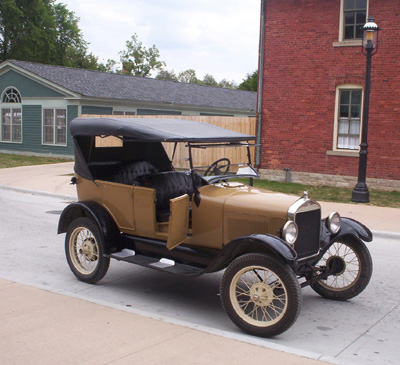
\includegraphics[width=.8\linewidth]{images/Late_model_Ford_Model_T.jpg}
  \caption{Ford modelo T del 1927 -- de Rmhermen \cite{Ford2022}.}
  \label{fig:ford_model_t}
\end{figure}

Durante aquella época, el ``mejor'' mecanismo de descubrimiento de
problemas era con algunos medidores y, sobre todo, por intuición:
sonidos del motor, olores extraños, \dots

No fue hasta los años 60 en donde los vehículos empezaron a incorporar
distintas interfaces con métricas que podían informar sobre el estado del
vehículo. El gran ``bum'' llegó con la expansión de la computadora, en donde
por primera vez se vio factible introducir un pequeño ordenador de 
abordo en el sistema.

En estos primeros sistemas, se incluyen indicadores del nivel de combustible,
sistema de refrigeración, presión del aceite, velocidad del motor,
temperatura del motor y otra información relativa al combustible. El
primer modelo que se conoce que incluye estos sistemas de cara a la
población en general es el Volkswagen Tipo III, en 1969 (figura \ref{fig:volkswagen_t3}):

\begin{figure}[H]
  \centering
  \includegraphics[width=.9\linewidth]{images/volkswagen_t3.jpg}
  \caption{Volkswagen Tipo III, modelo de inyección de 1969 -- de OSX - Trabajo propio \cite{VolkswagenTipo2021}.}
  \label{fig:volkswagen_t3}
\end{figure}

Pese a que supusieron un gran avance, estos primeros sistemas de
diagnóstico daban una información muy valiosa pero limitada, ya que muchos
diagnósticos seguirían siendo mediante los sentidos y las sensaciones
que le transmitiese el vehículo al mecánico. No fue hasta 1980 en donde
se implementó de forma estándar en los vehículos de \textit{General Motors}
el \ac{ALDL}, un lector de errores del coche que funcionó inicialmente a
160 baudios. Años más tarde, el sistema se refinaría usando el estándar
\ac{UART} \textit{half--duplex}, es decir, transmisión en los dos sentidos pero
no de forma simultánea (figura \ref{fig:aldl}). La principal motivación de incluir estos sistemas no fue
otra sino intentar reducir la contaminación de los vehículos teniendo
acceso a esta información \cite{SistemaOBD2Historia}.

\begin{figure}[H]
  \centering
  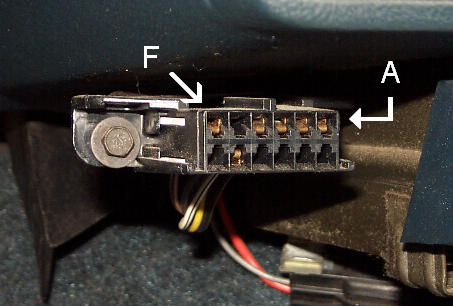
\includegraphics[width=.75\linewidth]{images/aldl.jpg}
  \caption{Conector \ac{ALDL}, creado por \textit{General Motors} antes de
  estandarizar OBD-II \cite{ReferenceManualChapter}.}
  \label{fig:aldl}
\end{figure}

No es hasta 1979 en que la \ac{SAE} recomienda crear un conector de
diagnóstico estandarizado en el mercado así como un conjunto de señales
de prueba. Finalmente, en 1991 la \ac{CARB} require que todos sus
vehículos tengan lo que sería el \ac{OBD}-I. Esta primera versión informaría
al conductor de un mal funcionamiento de alguno de los elementos del
vehículo mediante un \ac{MIL}, un indicador luminoso de fallos. Sin
embargo, solo se monitorizaban ciertos componentes relacionados con las
emisiones y no estaban calibrados \cite{SistemaOBD2Historia}.

Por ende, impulsado por las alertas \textit{smog} y por una fuerte regulación, en 1994
la \ac{CARB} obligó a todos los vehículos fabricados y vendidos a partir de 1996 incluir
el \ac{OBD}-II. Esto supuso un gran impulso en los mecanismos de monitorización de los
vehículos ya que además se estandarizó tanto el conector como los protocolos recomendados
por la \ac{SAE}. Tiempo más tarde, el Gobierno de los Estados Unidos aplicó la misma
medida a todos los vehículos del país \cite{SistemaOBD2Historia}.

Esta medida llegaría a Europa en 1998, según la Directiva 98/69EG, que obligaba a
todos los vehículos europeos a incluir dicho conector. Específicamente, los
automóviles de gasolina debían empezar a equiparlo en los modelos del año 2000; en el año 2003
para vehículos diésel; y en el año 2005 para camiones \cite{SistemaOBD2Historia}.

\subsection*{OBD--II}
\ac{OBD}--II es la segunda generación del sistema de diagnósticos de abordo, sucesor
de \ac{OBD}--I y su principal función es la de avisar al conductor cuando las
emisiones del vehículo son en torno a $1.5$ veces mayores de las diseñadas. A
diferencia de \ac{OBD}--I, \ac{OBD}--II también detecta fallos eléctricos, químicos
y mecánicos que puedan afectar al nivel de emisiones del vehículo (un caso típico
era un fallo químico del catalizador, indetectable por \ac{OBD}--I pero sí por la
segunda generación).

Este tipo de conector, al ser el primer estándar, cuenta con
múltiples interfaces que permiten conexiones mediante redes Wi-Fi, USB, Bluetooth,
etc. (cayendo pues en deshuso el protocolo de conexión por puerto serie -- RS232).
Esto se ha conseguido gracias al rápido avance de los sistemas embebidos, en donde
la combinación de \textit{software} y \textit{hardware} embebidos ha permitido que
cualquier usuario tenga acceso a este tipo de datos de forma relativamente simple
(actualmente, el conector más estandarizado es el controlador \texttt{ELM327} \cite{SistemaOBD2Historia},
figura \ref{fig:elm327}):

\begin{figure}[H]
  \centering
  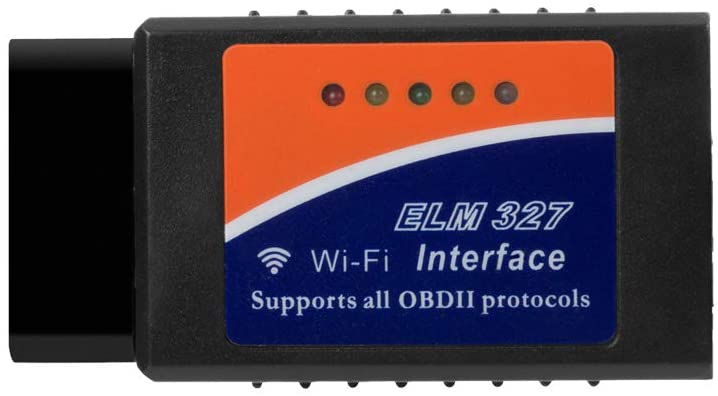
\includegraphics[width=.7\linewidth]{images/obd-ii-elm327.jpg}
  \caption{Controlador \texttt{ELM327} que cuenta con antenas Wi-Fi y Bluetooth para un acceso remoto \cite{AmazonComElm327}.}
  \label{fig:elm327}
\end{figure}

El sistema verifica todos los sensores directamente involucrados con las emisiones
del vehículo, como por ejemplo la inyección de aire al motor. Cuando algún sensor detecta
un fallo, se activa el \ac{MIL} indicando el fallo que sucede (o una combinación
de indicadores para notificar la existencia de un fallo, sin especificar exactamente
cuál).

El vehículo que incorpora un conector \ac{OBD}--II almacena la información sobre el
fallo del vehículo para que el mecánico que deba revisar el automóvil disponga de todos
los datos posibles. Por otra parte, este estándar permite una comunicación directa
con el vehículo mediante el envío de órdenes según un \ac{PID}. Por defecto, hay
una serie de \ac{PID}s estándar que la gran mayoría de vehículos deben incluir\footnote{%
Se dice ``la mayoría de vehículos'' porque hay ciertos \ac{PID}s que dependen
directamente del tipo de vehículo (a combustión, eléctrico, \dots) o del combustible
utilizado -- un vehículo eléctrico no ofrece información sobre las \ac{RPM} al igual
que un vehículo diésel no ofrece información sobre las bujías.}, pero también
los fabricantes de vehículos incluyen una serie de \ac{PID}s propios (conocidos como
\textit{\ac{PID}s propietarios}) que ofrecen información adaptada a cada vehículo
en particular y que, en principio, son privados y cerrados al público en general.

En Europa se implantó el \ac{EOBD}, la variación europea del estándar \ac{OBD}--II
implantada en el año 2000 en general. Si bien en apariencia es semejante al \ac{OBD}--II,
las diferencias radican en el \textit{software}. Por ejemplo, el estándar europeo
no monitoriza las evaporaciones del depósito de combustible; sin embargo, es más
sofisticado ya que usa ``mapas'' en las entradas de los sensores que obligan a que el
sensor se calibre empíricamente al sistema según las condiciones de operación del
motor (lo cual se traduce en que los sensores son mucho mejores pero más caros)
\cite{SistemaOBD2Historia}. Otra característica innovadora es que el sistema
europeo registra cuántos kilómetros se han recorrido desde que ha aparecido un
defecto \cite{EOBDOBD2}.

Finalmente, pero no menos importante, Japón tiene también su propio estándar denominado
\ac{JOBD}.

\subsection*{OBD--III}
El \ac{OBD}--III se espera que sea la siguiente versión del sistema que ya implementan
los coches actualmente. La principal diferencia con respecto a la versión anterior
será que el vehículo estará conectado de forma continua y emitiendo datos referentes
a las emisiones. De esta forma, se puede saber casi en el momento acerca de modificaciones
ilegales, un aumento en la contaminación del coche (signo de deterioro) y demás. No se
espera igualmente que sea un salto cualitativo ya que se sigue buscando que sea
altamente compatible con las herramientas que ya existen. Actualmente, se están
realizando pruebas en EE.UU. pero no hay cerrada ninguna fecha de estandarización
oficial por parte de los distintos continentes.

\subsection{Herramientas de monitorización y control del automóvil}
Pese al tiempo que lleva \ac{OBD}--II disponible, las herramientas existentes para
la actuación sobre un vehículo son relativamente escasas. La mayoría de modelos
presentes hoy en día en el mercado se basan directa o indirectamente en el
\texttt{ELM327}, un dispositivo de diagnóstico \ac{OBD} que cuenta con conexión
WiFi, Bluetooth y serie para la lectura local.

Por lo general, las herramientas que hay se utilizan por mecánicos o fanáticos del
sector para acceder a la información del estado del vehículo y ver los errores que
pudiera tener. Sin embargo, tras una breve documentación sobre el tema, la mayoría
de los casos buscaban directamente monitorizar en el momento el estado
del vehículo para obtener información relativa a los consumos, contaminación,
etc.

Por ejemplo, en el trabajo de Rimpas \textit{et al.} \cite{rimpasOBDIISensorDiagnostics2020}, se utiliza
un sensor \texttt{ELM327} para verificar que la información proporcionada por
el puerto del vehículo y la presentada por la telemetría presente en el mismo
(velocímetro y tacómetro) son coherentes entre sí (previa adaptación de los
valores en \textit{bytes} presentados por el conector a valores legibles). En
dicha investigación se llega a la conclusión de que el conector \ac{OBD}--II obtiene
valores fiables y consistentes tanto con los mostrados por el propio vehículo
como los proporcionados por el fabricante.

Otro tipo de investigaciones llevadas a cabo gracias a la presencia de este conector
en los automóviles es la de la caracterización de conductores y hábitos de conducción
según la telemetría reportada por el vehículo. En el estudio realizado por
Galih Hermawan y Emir Husni \cite{hermawanAcquisitionModelingEvaluating2020} se
estudia la combinación de la lectura de los sensores mediante el \ac{OBD}--II con
vehículos que presentan el sistema \ac{ADAS}.
El estudio busca identificar hábitos de conducción según la lectura de los diversos
sensores que hay en el sistema. También persigue detectar quién es el conductor que
está llevando el vehículo actualmente. En el estudio, el uso de \ac{OBD}--II junto
con los algoritmos de los \textit{k--Nearest Neighbor} (k--NN) y \textit{Naive Bayes}
consiguieron una precisión en la identificación del 100\% (
para un conjunto de datos de 10 conductores).
Por otra parte, el uso de inteligencia artificial junto con técnicas de \textit{clustering}
permitieron identificar comportamientos de los conductores al volante y relacionarlo
además con situaciones de riesgo y peligro. Además, se ha aplicado a otras características
también interesantes como detectar el tipo de calzada, predecir el tiempo de viaje,
analizar el consumo del vehículo y demás. El esquema seguido en la investigación es el
que se presenta en la figura \ref{fig:investigation-scheme}:

\begin{figure}[H]
  \centering
  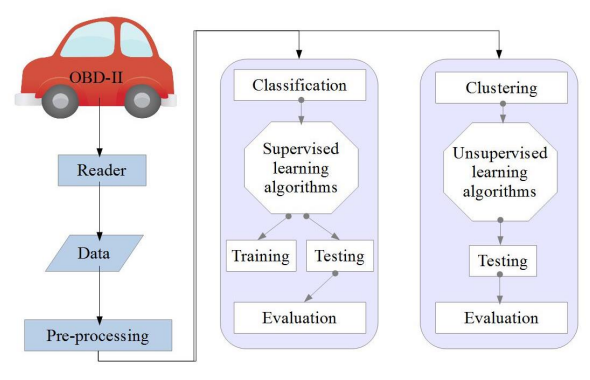
\includegraphics[width=.7\linewidth]{images/general-scheme-investigation.png}
  \caption{Esquema seguido para determinar los hábitos de conducción usando el \ac{OBD}--II \cite{hermawanAcquisitionModelingEvaluating2020}.}
  \label{fig:investigation-scheme}
\end{figure}

Por último, uno de los tipos de investigación bastante interesante realizada en los
últimos años es la de la generación de perfiles de conducción y de consumo. En el
artículo realizado por Ameen \textit{et al.} \cite{husseinaliameenDrivingBehaviourIdentification2021}
se define un sistema de clasificación del comportamiento del conductor al volante
(que es además el que se propone usar en este proyecto) el cual combina los datos
recibidos por el \ac{OBD}--II y del \ac{GPS} (figura \ref{fig:driving-behaviour}):

\begin{figure}[H]
  \centering
  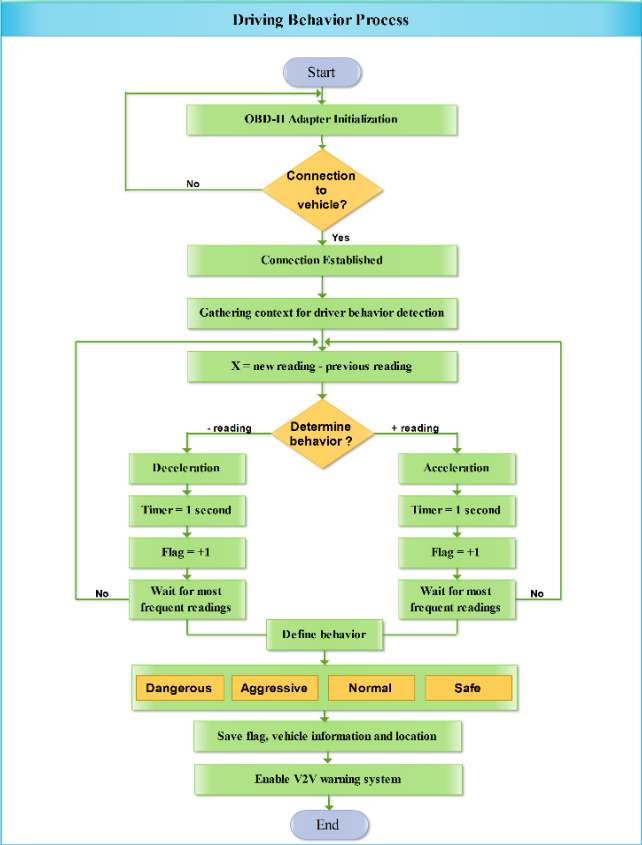
\includegraphics[width=.7\linewidth]{images/driving-behaviour-workflow.png}
  \caption{Flujo de análisis para determinar el comportamiento al volante de un conductor \cite{husseinaliameenDrivingBehaviourIdentification2021}.}
  \label{fig:driving-behaviour}
\end{figure}

Al final, el estudio concluía con los siguientes perfiles de conducción:

\begin{itemize}
  \item \textbf{Peligroso}, para una aceleración en general superior a $7\ \nicefrac{m}{s^2}$.
  \item \textbf{Agresivo}, para una aceleración entre $\left[4\ \nicefrac{m}{s^2}, 7\ \nicefrac{m}{s^2}\right)$.
  \item \textbf{Normal}, para una aceleración entre $\left[2\ \nicefrac{m}{s^2}, 4\ \nicefrac{m}{s^2}\right)$.
  \item \textbf{Seguro}, para una aceleración entre $\left[0\ \nicefrac{m}{s^2}, 2\ \nicefrac{m}{s^2}\right)$.
\end{itemize}

\section{Objetivos del desarrollo del proyecto}\label{sec:objectives}
Como se ha podido apreciar, existen multitud de aplicaciones relacionadas directa
o indirectamente con el \ac{OBD}--II, en parte por la longevidad del conector
en el mercado.

Sin embargo, todas o la gran mayoría de aplicaciones están destinadas a los profesionales
del sector, e incluso se ha aprovechado este conector para dificultar el acceso a
los datos del vehículo, habiendo de ir a un taller oficial para que puedan hacer
las reparaciones pertinentes.

Por otra parte, el parque de vehículos español es cada año más viejo debido a
diversos factores que no se van a analizar en este trabajo. Esto implica que cada
año más y más vehículos pierden el soporte por parte del fabricante y se vuelven
cada vez más costosos y complejos de mantener.

Para los no eruditos, el mundo del automóvil es el gran desconocido en donde una
serie de personas cualificadas se encargan del mantenimiento y correcto funcionamiento
del mecanismo que nos transporta por el mundo. Si bien es cierto que es necesaria
esta figura, hay una serie de buenas prácticas y actuaciones que pueden prevenir
tener que ir al mecánico de forma recurrente. Solo hace falta acceso a la información
de manera accesible.

Es por esto que nace \ac{VIMS}, un proyecto que pretende desarrollar un sistema completo
que consta de varias partes: un dispositivo embebido, un servidor y el usuario en sí
(figura \ref{fig:general-scheme}):

\begin{figure}[H]
  \centering
  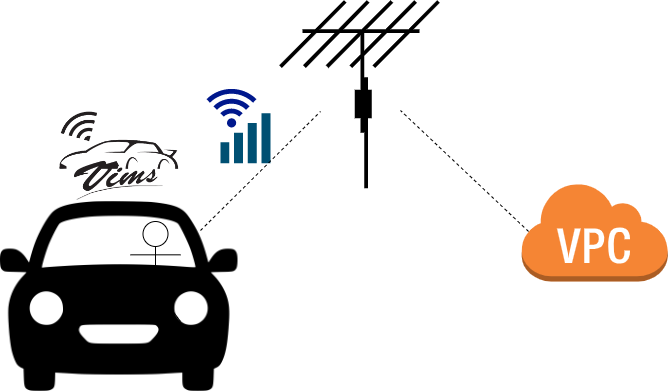
\includegraphics[width=\linewidth]{images/general-scheme.png}
  \caption{Esquema general que modela el modo de funcionamiento del sistema.}
  \label{fig:general-scheme}
\end{figure}

La idea fundamental detrás de este proyecto es la de devolverle a los usuarios
el control sobre su vehículo, ser conscientes de cómo funciona o, al menos, entender
mejor qué pueden hacer para mejorar tanto su estilo de conducción como la seguridad
al volante. De esta forma, con el dispositivo se espera también prevenir riesgos
ya que los propietarios y usuarios de los vehículos estarán informados en todo
momento de qué error pueda tener.

Como se prevé que este dispositivo sea utilizado por una gran variedad de usuarios
es crucial que sea accesible en términos de sencillez de manejo, entendimiento y
uso: evitar datos excesivamente técnicos, presentar la información más relevante
primero, etc.

Para ello, se hará uso de plataformas en la nube para gestionar, almacenar y presentar
la información al usuario y se contará con una aplicación móvil que permita un
fácil acceso a los datos del vehículo, tanto históricos como generados en el momento.

Al igual que otros trabajos previamente realizados, el proyecto se realiza sobre
las filosofías del código libre y del \textit{hardware} libre, que se traduce en
que todos los recursos (tanto físicos como \textit{software}) estarán disponibles
enteramente para cualquier persona interesada en ver cómo funciona, replicar el
proyecto por su cuenta y contar con plena potestad para mejorarlo, redistribuirlo
y trabajar con él (siempre bajo un prisma de reconocimiento al autor original
del trabajo regido por \textit{copyright}). Para ello, se ha decidido hacer uso
de la licencia MIT\footnote{Se pueden obtener más detalles sobre la licencia MIT
en la siguiente URL: \url{https://choosealicense.com/licenses/mit/}}.

\section{Metodología}\label{sec:methodology}
El proyecto que se pretende desarrollar es un proyecto de ingeniería. Esto se
traduce en que la metodología y la forma de trabajo son pilares fundamentales
en el desarrollo del mismo.

El primer paso realizado fue el de recopilar recursos e información de qué
necesitaban específicamente los usuarios. Para ello, se elaboró un cuestionario
en donde de forma general se preguntaba a conductores y no conductores qué querrían
tener en su vehículo. Los primeros sirvieron de grupo de control, los segundos para
aumentar la entropía de los datos obtenidos. El primer análisis realizado se detalla
en la sección \ref{ssec:user-req}, de la especificación de requisitos. Posteriormente,
en el punto \ref{chap:merch} se analiza en mayor profundidad los datos obtenidos
y se extraerán conclusiones.

A continuación, se realizó un estudio sobre qué plataformas y dispositivos están
accesibles de forma global para la generación y transmisión de datos. Esta fase
se centró principalmente en ``descubrir'' variantes del modelo ESP32 que incluyesen
ciertas antenas para permitir una mayor conectividad. Tras valorar diversas opciones,
se decidió usar el LILYGO T-SIM7000G ESP32 que incluye soporte de forma nativa para
tarjetas microSD, antena \ac{LTE}, alimentación externa por batería, antena \ac{GPS}, WiFi y
Bluetooth.

Una vez se decidió que dispositivo físico se iba a utilizar, se comenzó con el desarrollo
de los distintos diagramas que modelan el sistema, tanto lógicos como de diseño. Esta
parte fue crucial para asentar las bases de lo que será el proyecto y ha permitido seguir
el avance del mismo.

Por último, se realizó el serigrafiado de la placa y se comenzó la implementación
física de los diseños realizados. Sin embargo, esta etapa no se ha podido completar
por distintos contratiempos que se comentan en más detalle en el punto \ref{chap:planification}.


%% Product description
\chapter{Estructura del proyecto}\label{chap:structure}
El desarrollo del sistema \ac{VIMS} es un proceso multidisciplinar en el que se deben
desarrollar varias áreas de conocimiento. Este proyecto se ha postulado como
un desarrollo integral de ingeniería y es por eso por lo que está dividido en
varios bloques que conforman un factor clave en el desarrollo del mismo.

En este proyecto existen diversos bloques diferenciados: un estudio de mercado y de
las características de los usuarios, un estudio matemático asociado a la lectura de
valores y adecuación del \textit{hardware}, el proceso de diseño \textit{hardware}
en sí, el diseño \textit{software} del sistema y el análisis de planificación del mismo.

\begin{itemize}
  \item El estudio de mercado pretende averiguar y formalizar las necesidades de los
  conductores y usuarios de la vía. Es la primera aproximación y facilita la
  delimitación del producto y, sobre todo, ofrecerle al usuario final algo de utilidad
  y que pueda necesitar.
  \item El estudio matemático se encarga de investigar la ``traducción'' de los
  valores recibidos por el vehículo (según los datos asociados al estudio de mercado
  realizado con anterioridad).
  \item El diseño \textit{software} modela principalmente cómo se va a estructurar
  el sistema y cómo debe comportarse ante los distintos eventos que puede recibir.
  Esta fase conlleva realizar diagramas lógicos y de diseño del sistema en su conjunto.
  \item El diseño \textit{hardware} conlleva tanto el estudio de los componentes del
  sistema así como de las restricciones físicas del mismo. Además, en esta sección
  también se introduce el diseño 3D de la caja que alojará la placa.
  \item El análisis de planificabilidad complementa el diseño \textit{software}
  y estudia si el sistema es planificable. En los requisitos no se define \ac{VIMS}
  como un sistema en tiempo real, pero la cantidad de componentes que contiene y las
  acciones que tiene que realizar requieren del uso de subrutinas y de una planificación
  previa para asegurar un correcto funcionamiento del mismo.
\end{itemize}

Es importante detallar que pese a que el sistema se compone de varios componentes,
son dos los principales que lo caracterizan:

\begin{enumerate}
  \item La placa, \ac{VIMS}, que va embebida en los vehículos del sistema. Se encarga
  de toda la lectura, adaptación y emisión de datos. Además, cuenta con soporte para
  poder realizar una transmisión de la información a un dispositivo asociado mediante
  redes \ac{PAN}.
  \item El servidor \textit{cloud}, el ``cerebro'' encargado de recibir las tramas,
  los datos y la información relativa a las placas \ac{VIMS}, los dispositivos de
  usuario y demás componentes. Además, tiene la responsabilidad de ofrecer a los
  usuarios una \ac{GUI}, generar información relevante a partir de los datos (como
  estadísticas), gestionar las suscripciones y enviar periódicamente la información
  al usuario.
\end{enumerate}

\section{Estudio de mercado}\label{sec:merch}
Para el desarrollo de este proyecto, se hizo un estudio de mercado tanto de los
consumidores como de sus características, además de una evaluación exhaustiva
de qué les gustaría tener en su vehículo.

Este proyecto pretende en un futuro salir a mercado y suplir características que los
usuarios echan en falta en sus correspondientes medios de transporte. Como en principio
funciona con cualquier vehículo que cuente con \ac{OBD}--II, las respuestas no se han
limitado a aquellos conductores que condujesen turismos sino cualquier tipo de
automóvil: motocicleta, camión, etc.

Es importante destacar que el estudio tiene varios sesgos que han restringido
y delimitado las respuestas que se han registrado:

\begin{enumerate}
  \item Se ha realizado un cuestionario usando Google Forms, una plataforma de Google
        que permite preparar una serie de preguntas y respuestas y aplicar ciertos
        filtros sobre ellas. Por ejemplo, para aquellos que dijeron ser conductores,
        se hicieron preguntas diferentes frente a quienes no lo fueran.

        Esto permite obtener datos más fidedignos y acotados según la población que
        respondiera. Sin embargo, tiene una limitación implícita: restringe el acceso
        a aquellos con conocimientos ``suficientes'' acerca de la plataforma. Pese
        a que el producto pretende ser lo más accesible posible, no hay que olvidar
        que este tipo de tecnologías permanecen desconocidas para una gran parte
        de la población con escasos conocimientos acerca de Internet o de las
        nuevas tecnologías. Se comentará más adelante, pero esto se ve reflejado
        principalmente en la edad media de quienes respondieron el cuestionario.

        Por otra parte, al ser un cuestionario aparece otra limitación implícita
        y es la validación y verificación de las respuestas: se confía en la buena
        fe de los participantes y en la calidad de sus respuestas. Igualmente, se
        desarrolló el cuestionario junto con una psicóloga que ayudó a definir
        preguntas cerradas e incluir ciertas respuestas de control. Por otra parte,
        se usó el propio mecanismo que ofrece este servicio de Google para ordenar
        aleatoriamente las respuestas del cuestionario (y que eso sirviese también
        como control).

  \item Los encuestados fueron contactados principalmente por la red social Twitter,
        mediante la difusión con ``me gusta'' y ``retweet''. También se usaron otros
        medios de comunicación (como el correo UPM y Telegram/WhatsApp), pero el
        mayoritario fue el ya mencionado. Nuevamente, esto introduce un sesgo tanto
        por edad como por accesibilidad.

  \item Junto con la encuesta, se realizó un sorteo entre aquellos que respondiesen
        a la misma de un cheque regalo de Amazon valorado en 20\EUR{}. Si bien este
        incentivo pudiera resultar interesante, puede resultar también en un nuevo
        sesgo en donde personas que o bien no compren en Amazon o bien no sepan
        lo que es no quisieran hacer el cuestionario.

        Además, se plantea la casuística en que ciertas personas quisieran responder
        al cuestionario solo por el cheque de Amazon, sin importar la calidad de
        las respuestas, ``ensuciando'' los resultados obtenidos y quitándole credibilidad
        al cuestionario en sí.

        Esto se analizará posteriormente junto con las respuestas recibidas y las
        preguntas de control introducidas.

  \item El cuestionario, al ser relativamente exhaustivo, pudo echar para atrás a muchos
        posibles encuestados ya que se estima que el tiempo medio para realizarlo es del
        orden de 10/15 minutos. A parte del daño evidente de tener menos muestra con la
        que trabajar, este posible suceso reduciría también la variedad de la población
        y la calidad del estudio realizado.
\end{enumerate}

La primera pregunta que se realizó a los encuestados era si eran conductores o no.
Los datos revelan que el $72.7\%$ ($16$) de los encuestados son conductores, mientras que el
$27.3\%$ ($6$) restantes no, del total que fueron $22$ (figura \ref{fig:drivers-nodrivers}):

\begin{figure}[H]
  \centering
  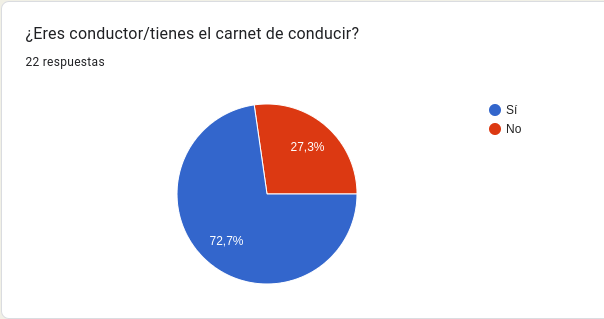
\includegraphics[width=\linewidth]{images/drivers-nodrivers.png}
  \caption{Gráfico de tarta que muestra quiénes de los encuestados son conductores ($72.7\%$) y quiénes no ($27.3\%$).}
  \label{fig:drivers-nodrivers}
\end{figure}

Sobre aquellos que dijeron ser conductores, se preguntó acerca de los años que
llevaban con carnet de conducir, así como los tipos de carnet de conducir que tenían
los encuestados.

Se vio que un $68.8\%$ tenía el carnet desde hace 3 años o más ($11$ encuestados
en particular); un $12.5\%$ tenía el carnet desde hace solo un año ($2$ encuestados)
y el restante, en su mayoría, tenía el carnet desde hace menos de un año. Esto se ve
reflejado en el histograma \ref{fig:carnet-time-hist}:

\begin{figure}[H]
  \centering
  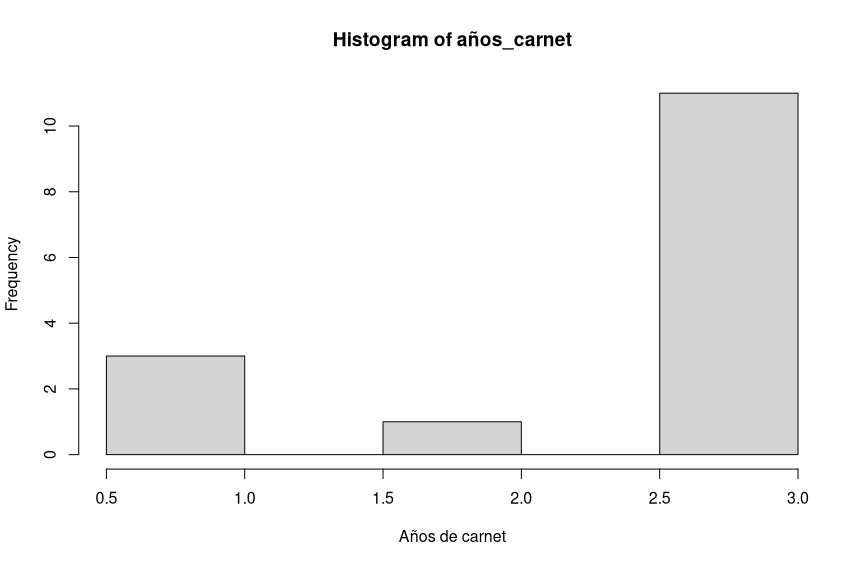
\includegraphics[width=\linewidth]{images/carnet-time.png}
  \caption{Histograma que muestra los años de carnet de los encuestados.}
  \label{fig:carnet-time-hist}
\end{figure}

Con respecto a los tipos de carnet, el $100\%$ de los encuestados (que dijeron ser
conductores) tiene el carnet tipo B. Se vio además que el $18.8\%$ tiene además los
carnets relativos a las motocicletas (muy posiblemente, los encuestados tienen el
carnet tipo ``A'' que les habilita automáticamente para aquellos de menor nivel,
como el AM, A1 y A2); y únicamente un encuestado tiene el carnet tipo C, que permite
conducir camiones.

Una restricción que se comentó con anterioridad era la edad media de los participantes.
Esta pregunta se realizó por dos motivos:

\begin{enumerate}
  \item Definir estadísticamente la edad media de la población para una posterior evaluación
        de su longevidad y experiencia tanto en la conducción como en la posible
        compra-venta de vehículos.
  \item Diferenciar, definir y clasificar los encuestados por grupos de edad y descubrir
        posibles sesgos y restricciones en las respuestas para un posterior análisis
        sobre la causa de dichos sesgos y restricciones.
\end{enumerate}

Es necesario decir que solo se preguntó por la edad a aquellas personas que respondieron
afirmativamente a ser conductores. Esto se hizo así debido a que sus respuestas han
conformado el dato más relativo a la hora de realizar la investigación, y se hace así
también estadísticamente.

Se tiene pues que:

\begin{equation}\label{eq:ages}
  \left\{\begin{aligned}
    X_{min}               & = 19     \\
    \bar{X}               & = 30     \\
    Mediana\left(X\right) & = 26.5   \\
    S\left(X\right)       & = 10.564 \\
    X_{max}               & = 55
  \end{aligned}\right.
\end{equation}

Se construyó además un gráfico de tarta (figura \ref{fig:ages}) que muestra cómo
quedan distribuidas las edades de los participantes:

\begin{figure}[H]
  \centering
  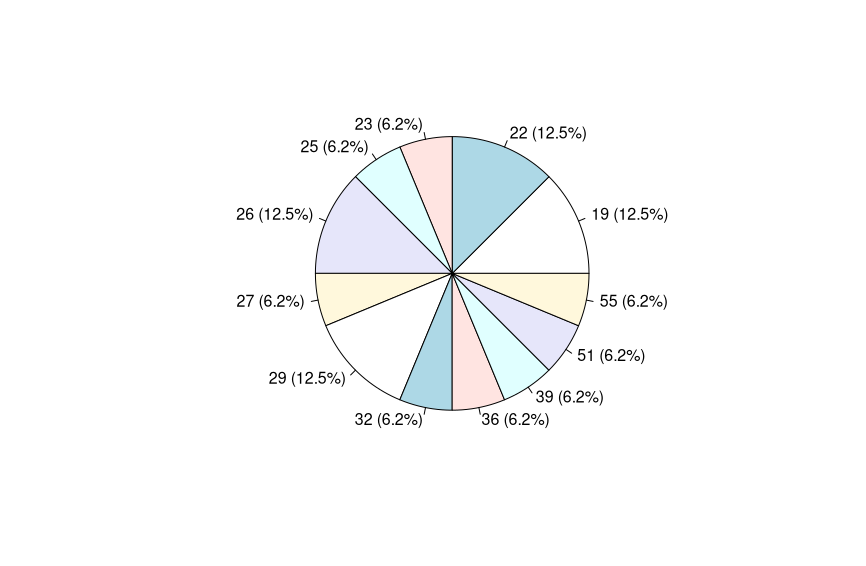
\includegraphics[width=\linewidth]{images/ages-pie.png}
  \caption{Gráfico de tarta que muestra la distribución de edades (valor previo al paréntesis) y su frecuencia en porcentaje.}
  \label{fig:ages}
\end{figure}

Como se puede ver en la ecuación \ref{eq:ages}, la distancia entre los valores
mínimo y máximo es de $36$ puntos. Sin embargo, los valores de la media $\left(\bar{X}\right)$
y la mediana $\left(Mediana\left(X\right)\right)$ muestran que la distribución está
bastante centrada en torno a la media, con una desviación estándar $\left(S\left(X\right)\right)$
de $\approx\pm10.564$.

Es interesante notar los tres grandes bloques presentes en la figura \ref{fig:ages}
que evidencian lo que se venía indicando anteriormente: en proporción, a la encuesta
ha accedido más población joven que adulta. Mismamente, solo el porcentaje de personas
encuestadas con edad por debajo de los 26 años es del $49.9\%$, casi la mitad de
los encuestados. Ampliando dicho margen hasta los 36 años, el porcentaje crece hasta
el $81 \%$.

Este dato se puede ver también reflejado en la distribución de los cuartiles, en donde
se tiene que:

\begin{equation}\label{eq:age-quartiles}
  \left\{
  \begin{aligned}
    Q_1 & = 22.75 \\
    Q_3 & = 33.00
  \end{aligned}
  \right.
\end{equation}

Como se puede apreciar en la ecuación \ref{eq:age-quartiles}, la distribución de
cuartiles está en un rango de edad por debajo de los 33 años para el $75\%$ de la
muestra, indicativo nuevamente de una población encuestada joven.

Destacan dos datos sobre los demás en donde los encuestados tienen 51 y 55 años
respectivamente. De este caso en particular se hablará posteriormente, pero cabe
destacar que sus respuestas fueron las más pobres en cuanto a contenido (sobre todo
en aquellas que sirvieron de control), seguramente debido al formato del
cuestionario, fatiga tras responder las secciones anteriores, etc.

Una vez se indagó acerca de la información que identifica a la muestra, se preguntó
directamente por el vehículo con el que contaban así como las características del
mismo. Para esta sección, se han dividido las preguntas en tres categorías:
\textit{básico}, \textit{habitual} y \textit{premium}. Dichas categorías se crean
según el porcentaje de uso habitual mundial de las características que se
enumeran en la tabla \ref{tab:car-specs}:

\begin{table}[H]
  \centering
  \begin{tabular}{|c|c|c|}
    \hline
    \textbf{Básico}          & \textbf{Habitual}            & \textit{\textbf{Premium}} \\
    \hline\hline
    Control de crucero       & Pantalla táctil              & Asistente virtual         \\
    Limitador de velocidad   & GPS                          & Aplicación móvil          \\
    Cámara de visión trasera & Detección de ángulos muertos & Cámara \textit{on-board}  \\
    Botón de arranque        & Android Auto                 &                           \\
    \hline
  \end{tabular}
  \caption{Tabla de distribución de las características de los vehículos, preguntado en el cuestionario.}
  \label{tab:car-specs}
\end{table}

Tras el cuestionario, las frecuencias obtenidas fueron:

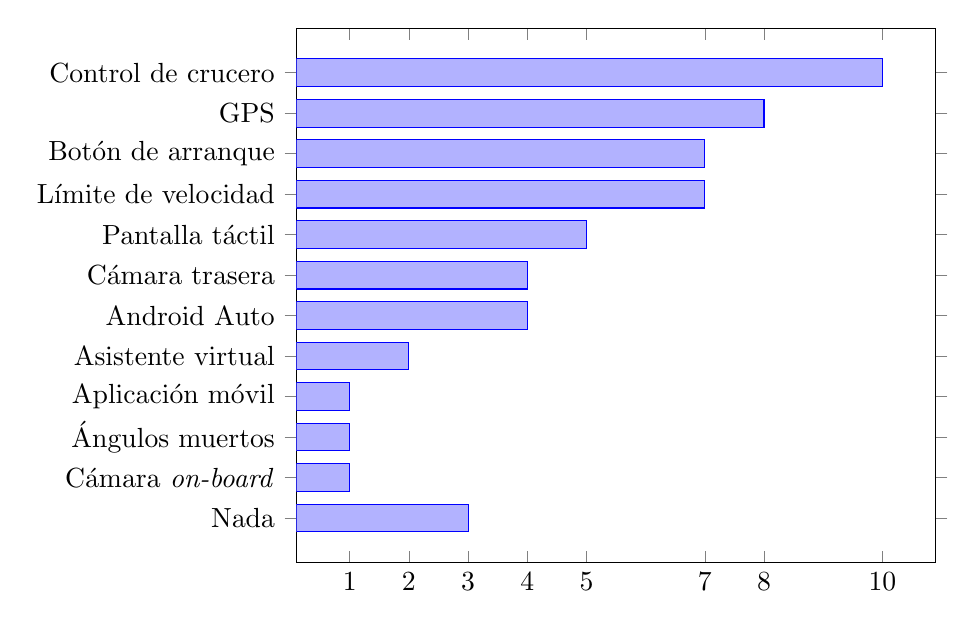
\begin{tikzpicture}
  \begin{axis} [%
      xbar,
      width=.8\linewidth,
      ytick=data,
      yticklabels={%
          Nada,
          Cámara \textit{on-board},
          Ángulos muertos,
          Aplicación móvil,
          Asistente virtual,
          Android Auto,
          Cámara trasera,
          Pantalla táctil,
          Límite de velocidad,
          Botón de arranque,
          GPS,
          Control de crucero,
        },
      xtick=data,
    ]
    \addplot coordinates {
        (3, 0)
        (1, 1)
        (1, 2)
        (1, 3)
        (2, 4)
        (4, 5)
        (4, 6)
        (5, 7)
        (7, 8)
        (7, 9)
        (8, 10)
        (10, 11)
      };
  \end{axis}
\end{tikzpicture}

\section{Estudio matemático}\label{sec:maths}
El estudio matemático va muy ligado al punto anterior (\ref{sec:merch}) ya que se
analizan los parámetros de \ac{OBD}--II y su ecuación matemática para obtener un
valor en $\mathbb{R}$ entendible por las personas.

Antes de dar paso a las ecuaciones en sí, es importante entender cómo funciona
el conector \ac{OBD}--II en esta situación. Los datos enviados y recibidos por
el coche están siempre codificados en un valor binario, recogido en un vector
de cuatro elementos en donde cada elemento tiene un \textit{byte} de tamaño. De
esta forma, se define al valor obtenido tras leer el conector \ac{OBD}--II como:

\begin{table}[H]
  \centering
  \resizebox{\textwidth}{!}{\begin{tabular}{|c|c|c|c|c|c|c|c|c|c|c|c|c|c|c|c|c|c|c|c|c|c|c|c|c|c|c|c|c|c|c|c|}
      \hline
      \multicolumn{8}{|c|}{$A$} & \multicolumn{8}{|c|}{$B$} & \multicolumn{8}{|c|}{$C$} & \multicolumn{8}{|c|}{$D$}                                                                                                                                                                                                                                 \\
      \hline
      $A_7$                     & $A_6$                     & $A_5$                     & $A_4$                     & $A_3$ & $A_2$ & $A_1$ & $A_0$ & $B_7$ & $B_6$ & $B_5$ & $B_4$ & $B_3$ & $B_2$ & $B_1$ & $B_0$ & $C_7$ & $C_6$ & $C_5$ & $C_4$ & $C_3$ & $C_2$ & $C_1$ & $C_0$ & $D_7$ & $D_6$ & $D_5$ & $D_4$ & $D_3$ & $D_2$ & $D_1$ & $D_0$ \\
      \hline
    \end{tabular}}
  \caption{Vector de \textit{bytes} que representa los datos recibidos del conector \ac{OBD}--II \cite{OBDIIPIDs2021}.}
  \label{tab:byte-array}
\end{table}

De esta forma, cuando se escribe $A_4$ se hace referencia al cuarto bit
del vector $A$. Los bits están ordenados según \ac{MSB}, de forma que
$A_7$ es el bit más significativo y $A_0$ el menor.

Los datos se obtienen del \ac{OBD}--II utilizando un lenguaje estándar llamado
\ac{PID}. El \ac{PID} se codifica como un número entero de 16 bits en donde los 8
primeros bits identifican el servicio/modo y los 8 restantes la operación a realizar.
Actualmente, están registrados los siguientes modos de funcionamiento (tabla
\ref{tab:pids-mode}):

\begin{table}[H]
  \centering
  \begin{tabularx}{\textwidth}{ | c | X | }
    \hline
    \textbf{Modo (hex)} & \textbf{Descripción}                                                                       \\
    \hline
    \texttt{01}         & Muestra los datos actuales del vehículo                                                    \\
    \hline
    \texttt{02}         & Muestra los datos almacenados del cuadro del vehículo                                      \\
    \hline
    \texttt{03}         & Muestra los códigos \ac{DTC}                                                               \\
    \hline
    \texttt{04}         & Elimina los códigos \ac{DTC} almacenados                                                   \\
    \hline
    \texttt{05}         & Resultados del test del sensor de oxígeno (sin \ac{CAN})                                   \\
    \hline
    \texttt{06}         & Resultados del test del sensor de oxígeno (con \ac{CAN})                                   \\
    \hline
    \texttt{07}         & Muestra los códigos \ac{DTC} pendientes (eliminados durante el último ciclo de conducción) \\
    \hline
    \texttt{08}         & Operaciones de control sobre los componentes del sistema                                   \\
    \hline
    \texttt{09}         & Petición de información sobre el vehículo                                                  \\
    \hline
    \texttt{0A}         & Códigos \ac{DTC} eliminados                                                                \\
    \hline
  \end{tabularx}
  \caption{Lista de modos de funcionamiento del estándar \ac{OBD}--II \cite{OBDIIPIDs2021}.}
  \label{tab:pids-mode}
\end{table}

Es importante destacar que no todos los fabricantes tienen por qué soportar todos
los modos, y que además ciertos fabricantes pueden definir sus modos propios por encima
del valor \texttt{09}.

Todos los modos definidos anteriormente tienen un conjunto de órdenes de soporte
en donde el sistema indica qué \ac{PID}s están soportados y cuáles no, por cada 32
\ac{PID}s. Por ejemplo, enviar la orden \texttt{0x0100} (\textit{modo 1, PID 0})
devolverá un valor que representará si los siguientes 32 \ac{PID}s están soportados.
Si el valor fuese, por ejemplo, \texttt{BE1FA813} se tendría que:

\begin{table}[H]
  \centering
  \resizebox{\textwidth}{!}{\begin{tabular}{ | c | c | c | c | c | c | c | c | c | c | c | c | c | c | c | c | c | c | c | c | c | c | c | c | c | c | c | c | c | c | c | c | c | }
      \hline
      \textbf{Hexadecimal} & \multicolumn{4}{|c|}{\texttt{B}} & \multicolumn{4}{|c|}{\texttt{E}} & \multicolumn{4}{|c|}{\texttt{1}} & \multicolumn{4}{|c|}{\texttt{F}} & \multicolumn{4}{|c|}{\texttt{A}} & \multicolumn{4}{|c|}{\texttt{8}} & \multicolumn{4}{|c|}{\texttt{1}} & \multicolumn{4}{|c|}{\texttt{3}}                                                                                                                                                                                                                                                                                                                                                 \\
      \hline
      \textbf{Binario}     & \texttt{1}                       & \texttt{0}                       & \texttt{1}                       & \texttt{1}                       & \texttt{1}                       & \texttt{1}                       & \texttt{1}                       & \texttt{0}                       & \texttt{0}  & \texttt{0}  & \texttt{0}  & \texttt{1}  & \texttt{1}  & \texttt{1}  & \texttt{1}  & \texttt{1}  & \texttt{1}  & \texttt{0}  & \texttt{1}  & \texttt{0}  & \texttt{1}  & \texttt{0}  & \texttt{0}  & \texttt{0}  & \texttt{0}  & \texttt{0}  & \texttt{0}  & \texttt{1}  & \texttt{0}  & \texttt{0}  & \texttt{1}  & \texttt{1}  \\
      \hline
      \textbf{?`Soportado?} & \done                            & \wontfix                         & \done                            & \done                            & \done                            & \done                            & \done                            & \wontfix                         & \wontfix    & \wontfix    & \wontfix    & \done       & \done       & \done       & \done       & \done       & \done       & \wontfix    & \done       & \wontfix    & \done       & \wontfix    & \wontfix    & \wontfix    & \wontfix    & \wontfix    & \wontfix    & \done       & \wontfix    & \wontfix    & \done       & \done       \\
      \hline
      \textbf{PID}         & \texttt{01}                      & \texttt{02}                      & \texttt{03}                      & \texttt{04}                      & \texttt{05}                      & \texttt{06}                      & \texttt{07}                      & \texttt{08}                      & \texttt{09} & \texttt{0A} & \texttt{0B} & \texttt{0C} & \texttt{0D} & \texttt{0E} & \texttt{0F} & \texttt{10} & \texttt{11} & \texttt{12} & \texttt{13} & \texttt{14} & \texttt{15} & \texttt{16} & \texttt{17} & \texttt{18} & \texttt{19} & \texttt{1A} & \texttt{1B} & \texttt{1C} & \texttt{1D} & \texttt{1E} & \texttt{1F} & \texttt{20} \\
      \hline
    \end{tabular}}
  \caption{Obtención de los \ac{PID}s soportados según el modo \cite{OBDIIPIDs2021}.}
  \label{tab:supported-pids}
\end{table}

A continuación, se dejan un conjunto de \ac{PID}s que se van a implementar en el
proyecto así como el código de acceso a ellos y la ecuación que permite obtener el
valor real.

\subsection*{Modo \texttt{01}}
Este modo permite acceder a la información en tiempo real del vehículo, según se
está en marcha. Los datos a los que se accede son:

\begin{table}[H]
  \centering
  \begin{tabularx}{\textwidth}{|c|X|}
    \hline
    \textbf{PID (hex)}       & \texttt{04}                    \\
    \hline
    \textbf{Bytes devueltos} & $1$                            \\
    \hline
    \textbf{Descripción}     & Carga del motor, en porcentaje \\
    \hline
    \textbf{Valor mínimo}    & $0\%$                          \\
    \hline
    \textbf{Valor máximo}    & $100\%$                        \\
    \hline
    \textbf{Fórmula}         &                                %
    \begin{equation*}
      \frac{A}{2.55}
    \end{equation*}                                 \\
    \hline
  \end{tabularx}
  \caption{\ac{PID} \texttt{04} -- carga del motor, en $\%$.}
\end{table}

\begin{table}[H]
  \centering
  \begin{tabularx}{\textwidth}{|c|X|}
    \hline
    \textbf{PID (hex)}       & \texttt{05}                            \\
    \hline
    \textbf{Bytes devueltos} & $1$                                    \\
    \hline
    \textbf{Descripción}     & Temperatura del refrigerante del motor \\
    \hline
    \textbf{Valor mínimo}    & $-40~\tccentigrade$                    \\
    \hline
    \textbf{Valor máximo}    & $215~\tccentigrade$                    \\
    \hline
    \textbf{Fórmula}         &                                        %
    \begin{equation*}
      A - 40
    \end{equation*}                                         \\
    \hline
  \end{tabularx}
  \caption{\ac{PID} \texttt{05} -- temperatura del refrigerante del motor, en $\tccentigrade$.}
\end{table}

\begin{table}[H]
  \centering
  \begin{tabularx}{\textwidth}{|c|X|}
    \hline
    \textbf{PID (hex)}       & \texttt{0C}         \\
    \hline
    \textbf{Bytes devueltos} & $2$                 \\
    \hline
    \textbf{Descripción}     & Velocidad del motor \\
    \hline
    \textbf{Valor mínimo}    & $0~RPM$             \\
    \hline
    \textbf{Valor máximo}    & $16383.75~RPM$      \\
    \hline
    \textbf{Fórmula}         &                     %
    \begin{equation*}
      \frac{256A + B}{4}
    \end{equation*}                      \\
    \hline
  \end{tabularx}
  \caption{\ac{PID} \texttt{0C} -- velocidad del motor, en $RPM$.}
\end{table}

\begin{table}[H]
  \centering
  \begin{tabularx}{\textwidth}{|c|X|}
    \hline
    \textbf{PID (hex)}       & \texttt{0D}            \\
    \hline
    \textbf{Bytes devueltos} & $1$                    \\
    \hline
    \textbf{Descripción}     & Velocidad del vehículo \\
    \hline
    \textbf{Valor mínimo}    & $0~\nicefrac{km}{h}$   \\
    \hline
    \textbf{Valor máximo}    & $255~\nicefrac{km}{h}$ \\
    \hline
    \textbf{Fórmula}         &                        %
    \begin{equation*}
      A
    \end{equation*}                         \\
    \hline
  \end{tabularx}
  \caption{\ac{PID} \texttt{0D} -- velocidad del vehículo, en $\nicefrac{km}{h}$.}
\end{table}

\begin{table}[H]
  \centering
  \begin{tabularx}{\textwidth}{|c|X|}
    \hline
    \textbf{PID (hex)}       & \texttt{11}             \\
    \hline
    \textbf{Bytes devueltos} & $1$                     \\
    \hline
    \textbf{Descripción}     & Posición del acelerador \\
    \hline
    \textbf{Valor mínimo}    & $0\%$                   \\
    \hline
    \textbf{Valor máximo}    & $100\%$                 \\
    \hline
    \textbf{Fórmula}         &                         %
    \begin{equation*}
      \frac{A}{2.55}
    \end{equation*}                          \\
    \hline
  \end{tabularx}
  \caption{\ac{PID} \texttt{11} -- posición del acelerador, en $\%$.}
\end{table}

\begin{table}[H]
  \centering
  \begin{tabularx}{\textwidth}{|c|X|}
    \hline
    \textbf{PID (hex)}       & \texttt{2F}                      \\
    \hline
    \textbf{Bytes devueltos} & $1$                              \\
    \hline
    \textbf{Descripción}     & Nivel del tanque del combustible \\
    \hline
    \textbf{Valor mínimo}    & $0\%$                            \\
    \hline
    \textbf{Valor máximo}    & $100\%$                          \\
    \hline
    \textbf{Fórmula}         &                                  %
    \begin{equation*}
      \frac{A}{2.55}
    \end{equation*}                                   \\
    \hline
  \end{tabularx}
  \caption{\ac{PID} \texttt{2F} -- nivel del tanque del combustible, en $\%$.}
\end{table}

\begin{table}[H]
  \centering
  \begin{tabularx}{\textwidth}{|c|X|}
    \hline
    \textbf{PID (hex)}       & \texttt{46}          \\
    \hline
    \textbf{Bytes devueltos} & $1$                  \\
    \hline
    \textbf{Descripción}     & Temperatura ambiente \\
    \hline
    \textbf{Valor mínimo}    & $-40~\tccentigrade$  \\
    \hline
    \textbf{Valor máximo}    & $215~\tccentigrade$  \\
    \hline
    \textbf{Fórmula}         &                      %
    \begin{equation*}
      A - 40
    \end{equation*}                      \\
    \hline
  \end{tabularx}
  \caption{\ac{PID} \texttt{46} -- temperatura ambiente, en $\tccentigrade$.}
\end{table}

\begin{table}[H]
  \centering
  \begin{tabularx}{\textwidth}{|c|X|}
    \hline
    \textbf{PID (hex)}       & \texttt{5B}                           \\
    \hline
    \textbf{Bytes devueltos} & $1$                                   \\
    \hline
    \textbf{Descripción}     & Tiempo restante de la batería híbrida \\
    \hline
    \textbf{Valor mínimo}    & $0\%$                                 \\
    \hline
    \textbf{Valor máximo}    & $100\%$                               \\
    \hline
    \textbf{Fórmula}         &                                       %
    \begin{equation*}
      \frac{A}{2.55}
    \end{equation*}                                       \\
    \hline
  \end{tabularx}
  \caption{\ac{PID} \texttt{5B} -- tiempo restante de la batería híbrida, en $\%$.}
\end{table}

\begin{table}[H]
  \centering
  \begin{tabularx}{\textwidth}{|c|X|}
    \hline
    \textbf{PID (hex)}       & \texttt{5C}            \\
    \hline
    \textbf{Bytes devueltos} & $1$                    \\
    \hline
    \textbf{Descripción}     & Temperatura del aceite \\
    \hline
    \textbf{Valor mínimo}    & $-40~\tccentigrade$    \\
    \hline
    \textbf{Valor máximo}    & $215~\tccentigrade$    \\
    \hline
    \textbf{Fórmula}         &                        %
    \begin{equation*}
      A - 40
    \end{equation*}                        \\
    \hline
  \end{tabularx}
  \caption{\ac{PID} \texttt{5C} -- temperatura del aceite, en $\tccentigrade$.}
\end{table}

\begin{table}[H]
  \centering
  \begin{tabularx}{\textwidth}{|c|X|}
    \hline
    \textbf{PID (hex)}       & \texttt{5E}               \\
    \hline
    \textbf{Bytes devueltos} & $2$                       \\
    \hline
    \textbf{Descripción}     & Consumo actual del motor  \\
    \hline
    \textbf{Valor mínimo}    & $0~\nicefrac{l}{h}$       \\
    \hline
    \textbf{Valor máximo}    & $3212.75~\nicefrac{l}{h}$ \\
    \hline
    \textbf{Fórmula}         &                           %
    \begin{equation*}
      \frac{256A + B}{20}
    \end{equation*}                           \\
    \hline
  \end{tabularx}
  \caption{\ac{PID} \texttt{5E} -- consumo actual del motor, en $\nicefrac{L}{h}$.}
\end{table}

\begin{table}[H]
  \centering
  \begin{tabularx}{\textwidth}{|c|X|}
    \hline
    \textbf{PID (hex)}       & \texttt{61}                       \\
    \hline
    \textbf{Bytes devueltos} & $1$                               \\
    \hline
    \textbf{Descripción}     & Torque demandado por el conductor \\
    \hline
    \textbf{Valor mínimo}    & $-125\%$                          \\
    \hline
    \textbf{Valor máximo}    & $130\%$                           \\
    \hline
    \textbf{Fórmula}         &                                   %
    \begin{equation*}
      A - 125
    \end{equation*}                                   \\
    \hline
  \end{tabularx}
  \caption{\ac{PID} \texttt{61} -- torque demandado por el conductor, en $\%$.}
\end{table}

\begin{table}[H]
  \centering
  \begin{tabularx}{\textwidth}{|c|X|}
    \hline
    \textbf{PID (hex)}       & \texttt{62}             \\
    \hline
    \textbf{Bytes devueltos} & $1$                     \\
    \hline
    \textbf{Descripción}     & Torque actual del motor \\
    \hline
    \textbf{Valor mínimo}    & $-125\%$                \\
    \hline
    \textbf{Valor máximo}    & $130\%$                 \\
    \hline
    \textbf{Fórmula}         &                         %
    \begin{equation*}
      A - 125
    \end{equation*}                         \\
    \hline
  \end{tabularx}
  \caption{\ac{PID} \texttt{62} -- torque actual del motor, en $\%$.}
\end{table}

\begin{table}[H]
  \centering
  \begin{tabularx}{\textwidth}{|c|X|}
    \hline
    \textbf{PID (hex)}       & \texttt{63}                    \\
    \hline
    \textbf{Bytes devueltos} & $2$                            \\
    \hline
    \textbf{Descripción}     & Torque de referencia del motor \\
    \hline
    \textbf{Valor mínimo}    & $0~Nm$                  \\
    \hline
    \textbf{Valor máximo}    & $65535~Nm$              \\
    \hline
    \textbf{Fórmula}         &                                %
    \begin{equation*}
      256A + B
    \end{equation*}                                \\
    \hline
  \end{tabularx}
  \caption{\ac{PID} \texttt{63} -- torque de referencia del motor, en $Nm$.}
\end{table}

\begin{table}[H]
  \centering
  \begin{tabularx}{\textwidth}{|c|X|}
    \hline
    \textbf{PID (hex)}       & \texttt{A4}                \\
    \hline
    \textbf{Bytes devueltos} & $4$                        \\
    \hline
    \textbf{Descripción}     & Marcha actual del vehículo \\
    \hline
    \textbf{Valor mínimo}    & $0~\text{ratio}$           \\
    \hline
    \textbf{Valor máximo}    & $65535~\text{ratio}$       \\
    \hline
    \textbf{Fórmula}         &                            %
    \begin{equation*}
      \begin{aligned}
        A_1 & = 1 \Longrightarrow \text{soportado} \\
        R   & = \frac{256C + D}{1000}
      \end{aligned}
    \end{equation*}                            \\
    \hline
  \end{tabularx}
  \caption{\ac{PID} \texttt{A4} -- marcha actual del vehículo, en ratio.}
\end{table}

\begin{table}[H]
  \centering
  \begin{tabularx}{\textwidth}{|c|X|}
    \hline
    \textbf{PID (hex)}       & \texttt{A6}      \\
    \hline
    \textbf{Bytes devueltos} & $4$              \\
    \hline
    \textbf{Descripción}     & Odómetro         \\
    \hline
    \textbf{Valor mínimo}    & $0~km$           \\
    \hline
    \textbf{Valor máximo}    & $429496729.5~km$ \\
    \hline
    \textbf{Fórmula}         &                  %
    \begin{equation*}
      \frac{A\left(2^{24}\right) + B\left(2^{16}\right) + C\left(2^8\right) + D}{10}
    \end{equation*}                  \\
    \hline
  \end{tabularx}
  \caption{\ac{PID} \texttt{A6} -- odómetro, en $km$.}
\end{table}

\subsection*{Modo \texttt{03}}
El modo \texttt{03} devuelve los \ac{DTC} guardados de la sesión actual. Estos códigos
de diagnóstico representan los distintos errores que hay en el vehículo, con un conjunto
de bytes que los identifican.

Este modo, a diferencia de los otros, no requiere de un parámetro \ac{PID} sino que solo
se envía el servicio como identificador. Una petición al modo \texttt{03} devolverá una
lista de $n$ elementos en donde cada elemento ocupa 2 bytes (por ende, el tamaño
esperable de la trama es $2n$).

Los códigos de error se definen como un conjunto de 5 caracteres de la forma: ``\texttt{U0158}''.
El valor de los caracteres define así:

\begin{table}[H]
  \centering
  \begin{minipage}{.32\linewidth}
    \begin{tabularx}{\textwidth}{|C{.3}|C{.7}|}
      \hline
      $A_7$ - $A_6$ & \textbf{Primer caracter \ac{DTC}}                         \\
      \hline
      \texttt{00}             & \textbf{P} -- sistema de propulsión (\textit{powertrain}) \\
      \texttt{01}             & \textbf{C} -- chassis                                     \\
      \texttt{10}             & \textbf{B} -- cuerpo (\textit{body})                      \\
      \texttt{11}             & \textbf{U} -- comunicaciones (\textit{network})           \\
      \hline
    \end{tabularx}
  \end{minipage}
  \hfill
  \begin{minipage}{.32\linewidth}
    \begin{tabularx}{\textwidth}{|C{.3}|C{.7}|}
      \hline
      $A_5$ - $A_4$ & \textbf{Segundo caracter \ac{DTC}} \\
      \hline
      \texttt{00}             & \texttt{0}                         \\
      \texttt{01}             & \texttt{1}                         \\
      \texttt{10}             & \texttt{2}                         \\
      \texttt{11}             & \texttt{3}                         \\
      \hline
    \end{tabularx}
  \end{minipage}
  \hfill
  \begin{minipage}{.32\linewidth}
    \begin{tabularx}{\textwidth}{|C{.3}|C{.7}|}
      \hline
      $A_3$ - $A_0$ & \textbf{Tercer caracter \ac{DTC}} \\
      \hline
      \texttt{0000}             & \texttt{0}                        \\
      \texttt{0001}             & \texttt{1}                        \\
      \texttt{0010}             & \texttt{2}                        \\
      \texttt{0011}             & \texttt{3}                        \\
      \texttt{0100}             & \texttt{4}                        \\
      \texttt{0101}             & \texttt{5}                        \\
      \texttt{0110}             & \texttt{6}                        \\
      \texttt{0111}             & \texttt{7}                        \\
      \texttt{1000}             & \texttt{8}                        \\
      \texttt{1001}             & \texttt{9}                        \\
      \texttt{1010}             & \texttt{A}                        \\
      \texttt{1011}             & \texttt{B}                        \\
      \texttt{1100}             & \texttt{C}                        \\
      \texttt{1101}             & \texttt{D}                        \\
      \texttt{1110}             & \texttt{E}                        \\
      \texttt{1111}             & \texttt{F}                        \\
      \hline
    \end{tabularx}
  \end{minipage}
\end{table}

Los caracteres cuarto y quinto se corresponden a los bits $B_7$ -- $B_4$ y $B_3$ -- $B_0$
respectivamente, y siguen la notación hexadecimal (al igual que los bits $A_3$ -- $A_0$).

De esta forma, con el código ya extraído, se necesita mirar en una tabla de valores
\ac{DTC} para saber exactamente a qué error se corresponde. Una web muy interesante
es la de ``OBD-Codes.com'' \cite{OBDCodesComLeading}, en donde hay información tanto
de códigos \ac{DTC} estándar como de códigos propietarios. Mirando en la propia
web, el código \texttt{U0158} se correspondería a: ``\textit{Lost communication with
head-up display}''\footnote{En la propia web dan muchos detalles e información
extendida sobre el error en cuestión, al igual que procedimientos para poder
solucionar el problema -- \url{https://www.obd-codes.com/u0158}}.

\subsection*{Modo \texttt{09}}
El modo \texttt{09} devuelve información referente al vehículo en sí, no al estado
de los sensores o del propio vehículo. Algunos datos interesantes son:

\begin{table}[H]
  \centering
  \begin{tabularx}{\textwidth}{|c|X|}
    \hline
    \textbf{PID (hex)}       & \texttt{02}                    \\
    \hline
    \textbf{Bytes devueltos} & $17$                            \\
    \hline
    \textbf{Descripción}     & \ac{VIN} \\
    \hline
    \textbf{Fórmula}         & \ac{VIN} de 17 caracteres ASCII con \textit{padding} a la izquierda de caracteres nulos (\texttt{0x00}) si hace falta \\
    \hline
  \end{tabularx}
  \caption{\ac{PID} \texttt{02} -- \ac{VIN}.}
\end{table}

\begin{table}[H]
  \centering
  \begin{tabularx}{\textwidth}{|c|X|}
    \hline
    \textbf{PID (hex)}       & \texttt{0A}                    \\
    \hline
    \textbf{Bytes devueltos} & $20$                            \\
    \hline
    \textbf{Descripción}     & Nombre de la \ac{ECU} \\
    \hline
    \textbf{Fórmula}         & 20 caracteres ASCII con \textit{padding} a la derecha de caracteres nulos (\texttt{0x00}) \\
    \hline
  \end{tabularx}
  \caption{\ac{PID} \texttt{0A} -- nombre de la \ac{ECU}.}
\end{table}

\section{Diseño \textit{software}}\label{sec:software}
\section{Diseño \textit{hardware}}\label{sec:hardware}
\section{Análisis de planificabilidad}\label{sec:rt-analysis}

%% Requirements
\chapter{Especificación de requisitos}\label{chap:requirements}
%% Introduction
\input{base/abstract.tex}

\chapter{Introducción}\label{chap:intro}
\input{content/introduction/introduction.tex}
\section{Estado del arte}\label{sec:state_of_the_art}
\input{content/introduction/state_of_the_art.tex}
\section{Objetivos del desarrollo del proyecto}\label{sec:objectives}
\input{content/introduction/objectives.tex}
\section{Metodología}\label{sec:methodology}
\input{content/introduction/methodology.tex}

%% Product description
\chapter{Estructura del proyecto}\label{chap:structure}
\input{content/description/structure.tex}
\section{Estudio de mercado}\label{sec:merch}
\input{content/description/merch.tex}
\section{Estudio matemático}\label{sec:maths}
\input{content/description/maths.tex}
\section{Diseño \textit{software}}\label{sec:software}
\section{Diseño \textit{hardware}}\label{sec:hardware}
\section{Análisis de planificabilidad}\label{sec:rt-analysis}

%% Requirements
\chapter{Especificación de requisitos}\label{chap:requirements}
\input{RS/content/content.tex}

%% Hardware and software design
\chapter{Diagramas y diseño}\label{chap:design}
\section{Diagramas que modelan el sistema}\label{sec:sys-diagrams}
\section{Diseño \textit{hardware} del sistema}\label{sec:hardware-design}
\section{Diseño 3D del sistema}\label{sec:3d-design}
\section{Diseño \textit{software} del sistema}\label{sec:software-design}
\section{Planificación del sistema de tiempo real}\label{sec:rt-design}

\chapter{Planificación, costes y tiempo empleado}\label{chap:planification}
\section{Diagramas de Gantt}
\section{Coste de los materiales}
\section{Sueldos propuestos y costes obtenidos}
\section{Contratiempos y tiempo de desarrollo final}

\chapter{Conclusiones}\label{chap:conclussions}
\section{Conclusiones técnicas}
\section{Conocimientos adquiridos y nuevas competencias}
\section{Reflexión final}

\chapter{Trabajo pendiente y futuras líneas de trabajo}\label{chap:pending-work}


%% Hardware and software design
\chapter{Diagramas y diseño}\label{chap:design}
\section{Diagramas que modelan el sistema}\label{sec:sys-diagrams}
\section{Diseño \textit{hardware} del sistema}\label{sec:hardware-design}
\section{Diseño 3D del sistema}\label{sec:3d-design}
\section{Diseño \textit{software} del sistema}\label{sec:software-design}
\section{Planificación del sistema de tiempo real}\label{sec:rt-design}

\chapter{Planificación, costes y tiempo empleado}\label{chap:planification}
\section{Diagramas de Gantt}
\section{Coste de los materiales}
\section{Sueldos propuestos y costes obtenidos}
\section{Contratiempos y tiempo de desarrollo final}

\chapter{Conclusiones}\label{chap:conclussions}
\section{Conclusiones técnicas}
\section{Conocimientos adquiridos y nuevas competencias}
\section{Reflexión final}

\chapter{Trabajo pendiente y futuras líneas de trabajo}\label{chap:pending-work}


%% Hardware and software design
\chapter{Diagramas y diseño}\label{chap:design}
\section{Diagramas que modelan el sistema}\label{sec:sys-diagrams}
\section{Diseño \textit{hardware} del sistema}\label{sec:hardware-design}
\section{Diseño 3D del sistema}\label{sec:3d-design}
\section{Diseño \textit{software} del sistema}\label{sec:software-design}
\section{Planificación del sistema de tiempo real}\label{sec:rt-design}

\chapter{Planificación, costes y tiempo empleado}\label{chap:planification}
\section{Diagramas de Gantt}
\section{Coste de los materiales}
\section{Sueldos propuestos y costes obtenidos}
\section{Contratiempos y tiempo de desarrollo final}

\chapter{Conclusiones}\label{chap:conclussions}
\section{Conclusiones técnicas}
\section{Conocimientos adquiridos y nuevas competencias}
\section{Reflexión final}

\chapter{Trabajo pendiente y futuras líneas de trabajo}\label{chap:pending-work}


%% Hardware and software design
\chapter{Diagramas y diseño}\label{chap:design}
\section{Diagramas que modelan el sistema}\label{sec:sys-diagrams}
\section{Diseño \textit{hardware} del sistema}\label{sec:hardware-design}
\section{Diseño 3D del sistema}\label{sec:3d-design}
\section{Diseño \textit{software} del sistema}\label{sec:software-design}
\section{Planificación del sistema de tiempo real}\label{sec:rt-design}

\chapter{Planificación, costes y tiempo empleado}\label{chap:planification}
\section{Diagramas de Gantt}
\section{Coste de los materiales}
\section{Sueldos propuestos y costes obtenidos}
\section{Contratiempos y tiempo de desarrollo final}

\chapter{Conclusiones}\label{chap:conclussions}
\section{Conclusiones técnicas}
\section{Conocimientos adquiridos y nuevas competencias}
\section{Reflexión final}

\chapter{Trabajo pendiente y futuras líneas de trabajo}\label{chap:pending-work}
